\documentclass[a4paper,12pt]{monografia}
\usepackage{amsmath,amsthm,amsfonts,amssymb}
\usepackage{latexsym}
\usepackage[brazil]{babel}
\usepackage[utf8]{inputenc}
\usepackage{graphicx}
\usepackage{hyperref}
\usepackage[none]{hyphenat}
\usepackage[alf]{abntex2cite}
\usepackage{graphicx}	
\usepackage{float}
\usepackage{xcolor,colortbl}
\usepackage{longtable}
\usepackage{caption}

\renewcommand{\rmdefault}{phv} % Arial
\renewcommand{\sfdefault}{phv} % Arial

\captionsetup{%
figurewithin=none,
tablewithin=none,  
}
\addto\captionsbrazil{
\renewcommand{\tablename}{Quadro}
}
\tolerance=1
\emergencystretch=\maxdimen
\newcommand{\mc}[2]{\multicolumn{#1}{c}{#2}}
\definecolor{Gray}{gray}{0.85}
\definecolor{ballblue}{rgb}{0.13, 0.67, 0.8}
\newcolumntype{a}{>{\columncolor{Gray}}l}
\newcolumntype{b}{>{\columncolor{white}}c}
\begin{document}
%
%----------------- Título e Dados do Autor -----------------
\titulo{Sudo Loja: Sistema de Gerenciamento de Conteúdo Voltado ao E-Commerce}
\autor{João Marcos Ferreira} \nome{João Marcos} \ultimonome{Ferreira}
%
%---------- Informe o Curso e Grau -----
\tecnologo \curso{Análise e Desenvolvimento de Sistemas} \ano{2016}
\data{dd/MM/2016} % data da aprovação
\cidade{Cajazeiras/PB}
%
%----------Informações sobre a Instituição -----------------
\instituicao{Instituto Federal de Educação Ciência e Tecnologia da Paraíba} \sigla{IFPB}
\unidadeacademica{}
%
%-------- Informações obtidas na Biblioteca ----------------
%
% \CDU{123.45} \areas{Areas..}

\npaginas{55}  % total de páginas do trabalho
%------Nomes do Orientador, 1o. Examinador e 2o.
\orientador{Francisco Paulo de Freitas Neto}
\abrevttorientador{Prof. Msc}
\examinadorum{Examinador 1}
\examinadordois{Examinador 2}
\ttorientador{Orientador}
\ttexaminadorum{Examinador}
\ttexaminadordois{Examinador}
\maketitle
%----------------------------dedicatória--------------
\begin{dedicatoria}
Aos meus pais e irmãos.\\
Aos meus amigos\\
\end{dedicatoria}

%----------------------------Agradecimentos--------------
\agradecimento{Agradecimentos}
\noindent Primeiramente a Deus. O que seria de nós sem Ele?	\\
Aos meus pais que sempre me incentivaram e me ajudaram, sem eles não teria chegado até aqui.\\
Ao meu Orientador Francisco Paulo de Freitas Neto pela paciência, disponibilidade e por prestar toda a orientação e esclarecimentos necessários.\\
Aos meus tios Isabel e Alonso por me acolherem durante todos esses dias.\\
À minha namorada por estar sempre ao meu lado me encorajando\\
Aos meus amigos e todos os meus parentes pelo apoio.

\newpage

%--------Resumo em Português--------------
\resumo{Resumo} 

Na atualidade muitas pessoas preferem fazer suas compras em casa usando seu computador ou \textit{smartphone}, ao invés de se deslocarem até uma loja ou supermercado. Com um número de pedidos no \textit{e-commerce} aumentando cada vez mais e movimentando quantias cada vez maiores, percebe-se que é um mercado em ascensão. Os comerciantes da região ainda desconhecem ferramentas que facilitam a criação e gestão de uma loja virtual. Este trabalho apresenta uma ferramenta capaz de criar, gerenciar e personalizar uma loja virtual. O uso desta ferramenta trará benefícios a aqueles interessados em vender na Internet, pois poderão com facilidade, sem burocracias, sem custos elevados, e sem precisar ter conhecimentos avançados sobre programação, criar e gerir seu próprio \textit{e-commerce}.

\noindent \textbf{Palavras-chaves:} Sistemas de Gerenciamento de Conteúdo. Loja Virtual. Vendas.
%-----------Resumo em Inglês--------------
\resumo{Abstract} 

Nowadays many people prefer to do their shopping at home using your computer or smartphone, instead of moving to a store or supermarket. With a number of requests in e-commerce continually increasing and moving increasingly larger amounts, it is clear that it is a growing market. Traders in the region are still unaware of tools that facilitate the creation and management of a virtual store. This paper presents a tool to create, manage and customize a virtual store. Use of this tool will benefit those interested in selling on the Internet, they may easily, without bureaucracy, without high costs and without having advanced knowledge about programming, create and manage your own e-commerce.

\noindent \textbf{Keywords:} Content Management Syste. Virtual Store. Sales.
\newpage

%---------------------- EPÍGRAFE I (OPCIONAL)--------------
\begin{epigrafe}
“Pequenas oportunidades são muitas vezes o começo de grandes empreendimentos.”\\
\hfill Demóstenes
\end{epigrafe}

%----Sumário, lista de figuras, quadros------------
\addtocontents{toc}{\protect\setcounter{tocdepth}{-1}}


{% Lista de Figuras 
\let\oldnumberline\numberline%
\renewcommand{\numberline}{\figurename~\oldnumberline}%
\listoffigures%
\thispagestyle{empty}
}

\renewcommand\listtablename{Lista de Quadros}

{% Lista de Quadros
\let\oldnumberline\numberline%
\renewcommand{\numberline}{\tablename~\oldnumberline}%
\listoftables%
\thispagestyle{empty}
}

\addtocontents{toc}{\protect\setcounter{tocdepth}{2}}
\tableofcontents
%---------------------
% 
\chapter{Introdução} % (fold)
\label{cha:intro}
\setcounter{page}{1}

Comprar na Internet traz muitas vantagens para um consumidor. É possível fazer compras sempre que quiser e à hora que desejar, no conforto da sua casa. Não existem filas. As compras são feitas sem a utilização de dinheiro físico, proporcionando mais segurança ao cliente.  Além de diversas outras vantagens.

Para os comerciantes as vantagens também são muitas: o produto fica acessível aos clientes 24 horas por dia, todos os dias da semana; pessoas de todos os lugares podem ver o produto; não precisa de um espaço físico para expor os produtos; custo de investimento inicial mínimo; sem risco de assalto, entre outras.

Dados indicam que os consumidores virtuais demonstram altos índices de intenção de compra, ou seja, continuam consumindo apesar do estabelecimento de um cenário de crise, e pricipalmente na Internet, onde os preços geralmente são mais baratos, se compara-dos aos do varejo tradicional.

O \textit{WebShoppers} \citeonline{webshoppers}, relatório sólido e respeitado sobre o comércio eletrônico anualmente publicado, no qual são analisadas a evolução do \textit{e-commerce}, tendências, estimativas, as mudanças de comportamento e preferências dos e-consumidores, apresentou boas estatísticas sobre o \textit{e-commerce} no Brasil. A seguir veremos esses dados em forma de figuras e gráficos.

A figura \ref{figura:consumidores} apresenta a quantidade de e-consumidores ativos (pessoas que efetivaram pelo
menos uma compra virtual, ao longo de 2015). Percebe-se um crescimento, se comparada com anos anteriores. Em 2015, esse número chegou ao total de 39,1 milhões de consumidores.

\begin{figure}[H]
\centering
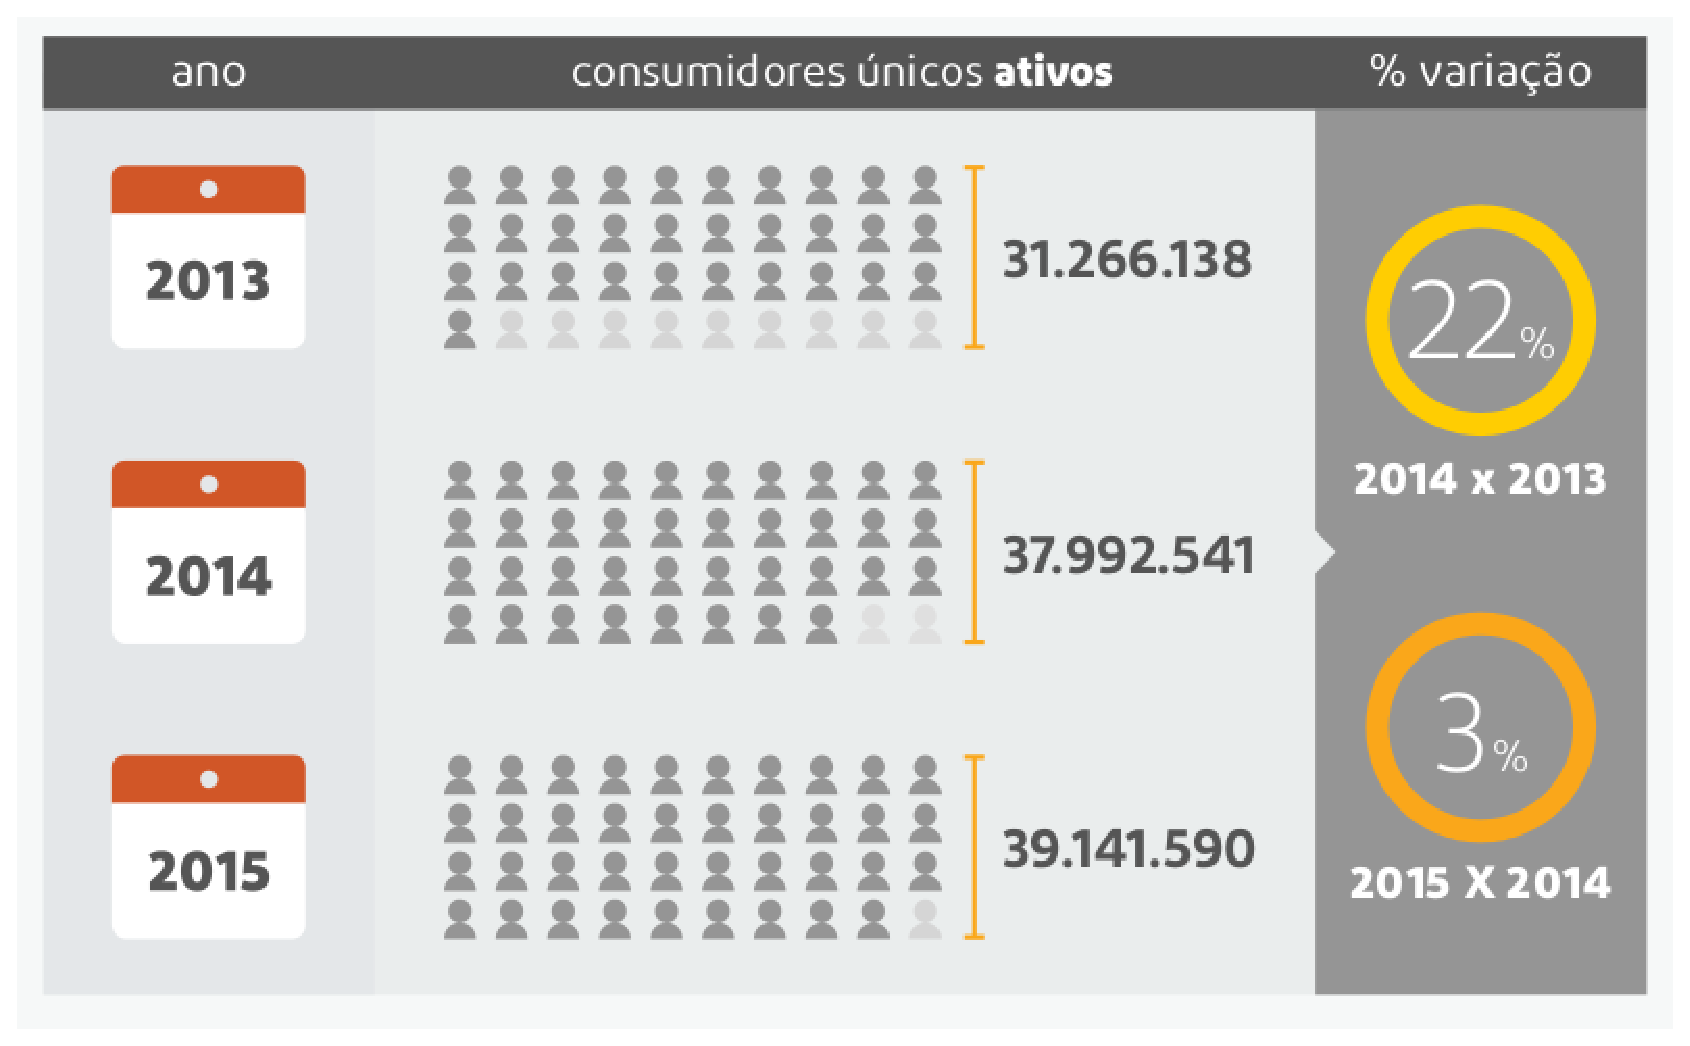
\includegraphics[width=12cm]{img/webshoppers/consumidores.eps}
\caption{Consumidores únicos ativos}
\small{Fonte: \citeonline{webshoppers} - Relatório WebShoppers}
\label{figura:consumidores}
\end{figure}

\begin{figure}[H]
\centering
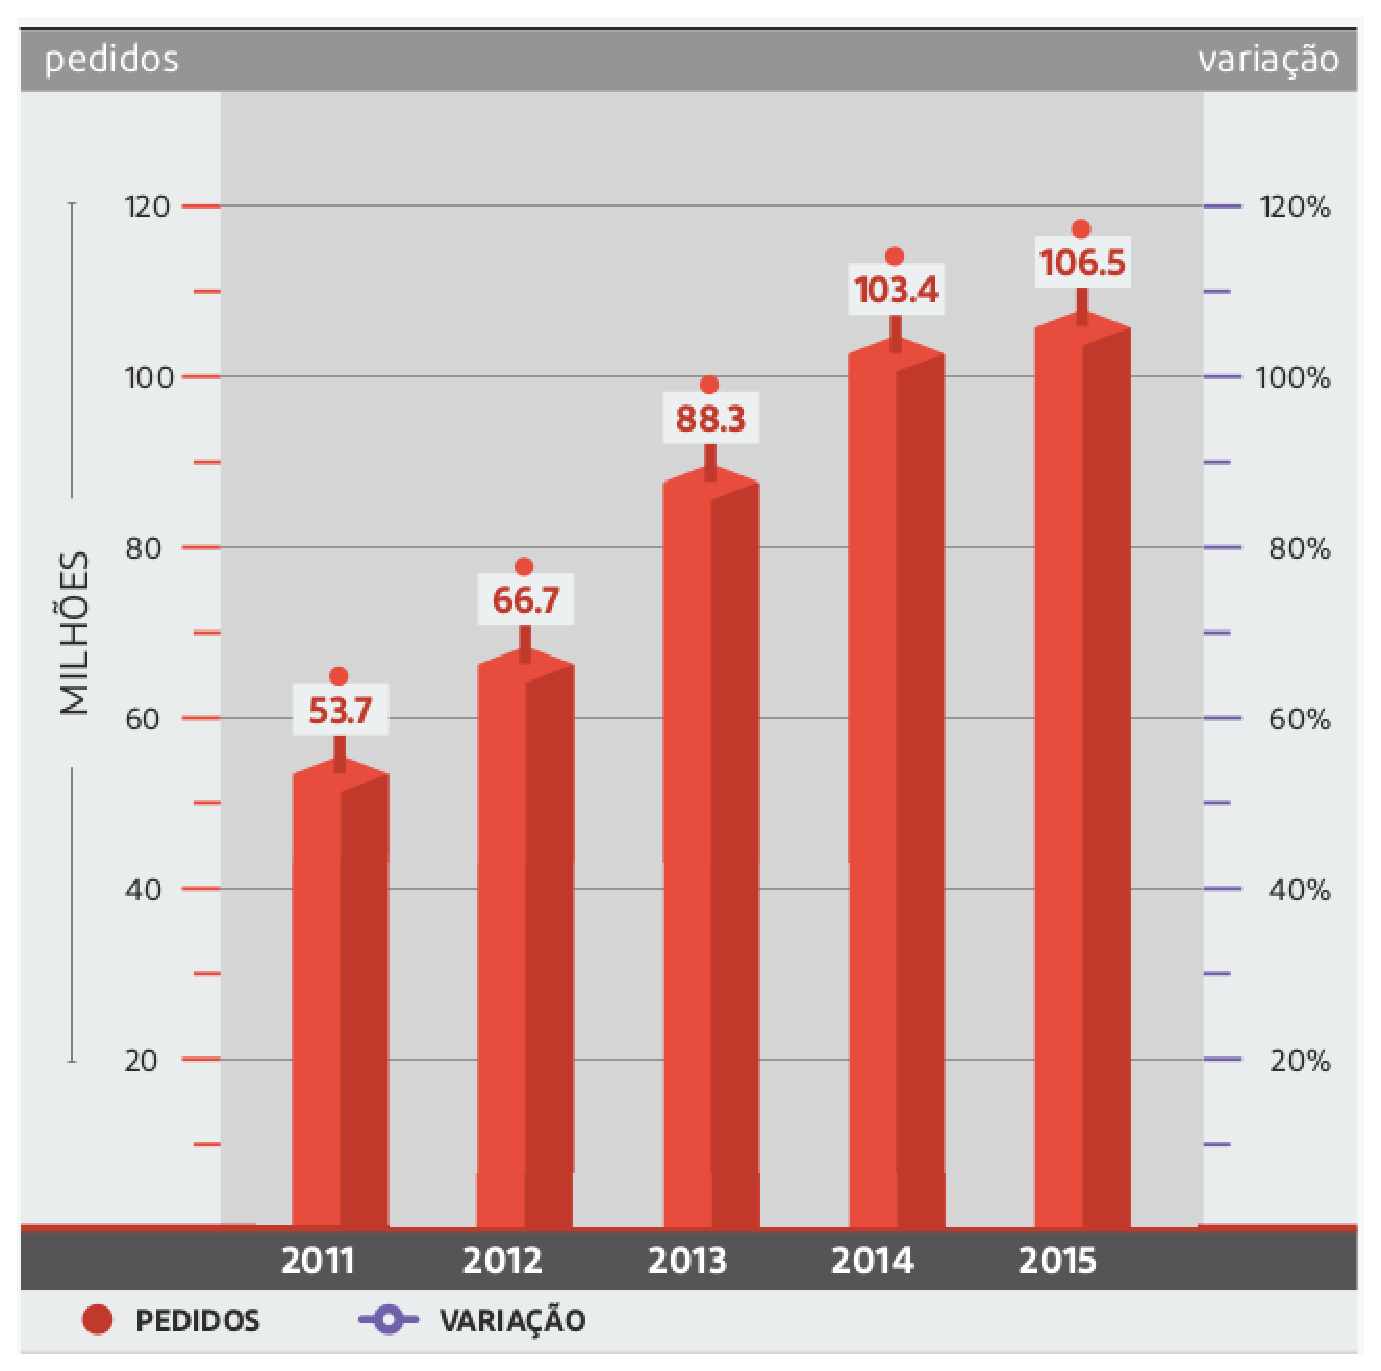
\includegraphics[width=10cm]{img/webshoppers/total-pedidos.eps}
\caption{Total de pedidos realizados no \textit{e-commerce} no Brasil}
\small{Fonte: \citeonline{webshoppers} - Relatório WebShoppers}
\label{figura:pedidos}
\end{figure}

O número de pedidos e o faturamento do comércio eletrônico também foram notavalmente altos. Como mostra a figura \ref{figura:pedidos}, com um total de 106,2 milhões em 2015, o incremento no número de pedidos no mercado brasileiro foi de 3\%, em relação a 2014. O faturamento do comércio eletrônico foi de R\$ 41,3 bilhões. O número representa um crescimento nominal de 15,3\%, em relação a 2014, quando as vendas somaram um total de R\$ 35,8 bilhões como pode ser visto na figura \ref{figura:vendas}.

\begin{figure}[H]
\centering
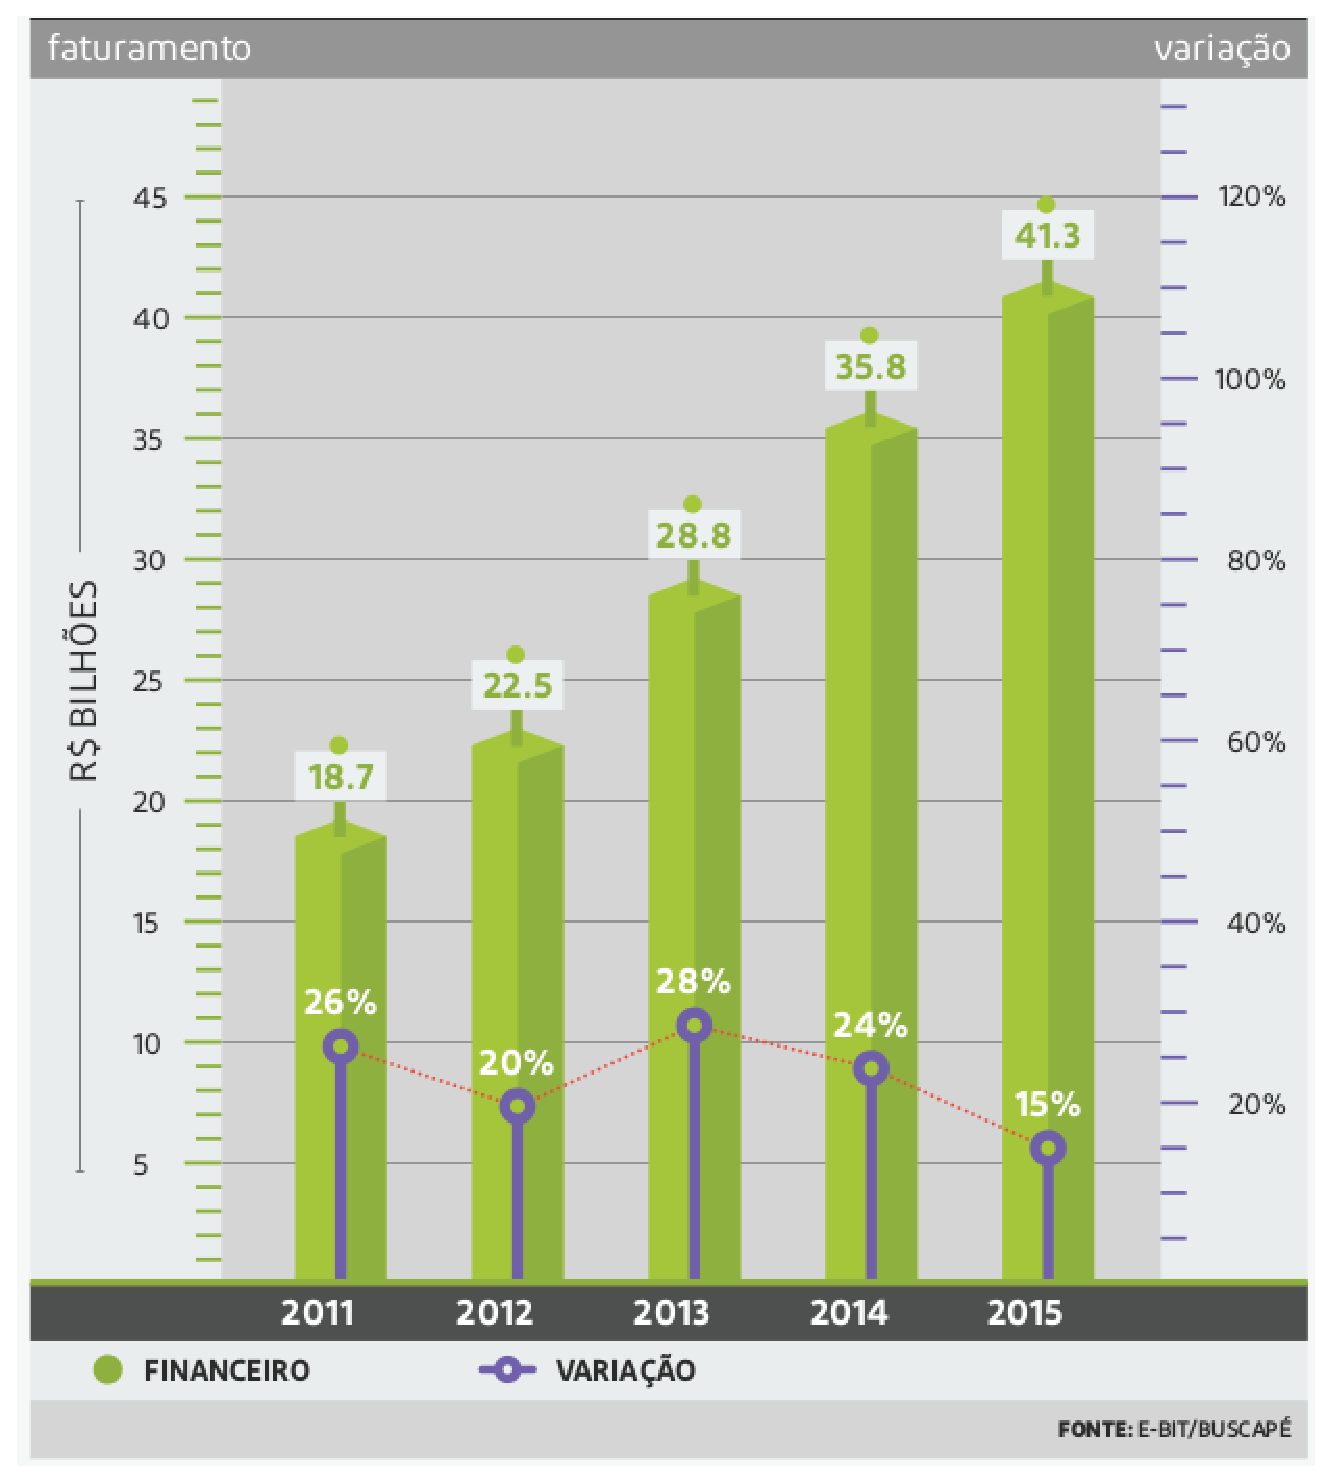
\includegraphics[width=10cm]{img/webshoppers/faturamento.eps}
\caption{Total de faturamento do \textit{e-commerce} no Brasil}
\small{Fonte: \citeonline{webshoppers} - Relatório WebShoppers}
\label{figura:vendas}
\end{figure}

O relatório também destaca dados sobre a satisfação dos clientes em realizar suas compras na internet. O Net Promoter Score (NPS) é um indicador que mensura a satisfação e a fidelização dos clientes. No balanço geral do ano, o NPS apresentou o melhor resultado. A figura \ref{figura:nps} apresenta esse dados.

\begin{figure}[H]
\centering
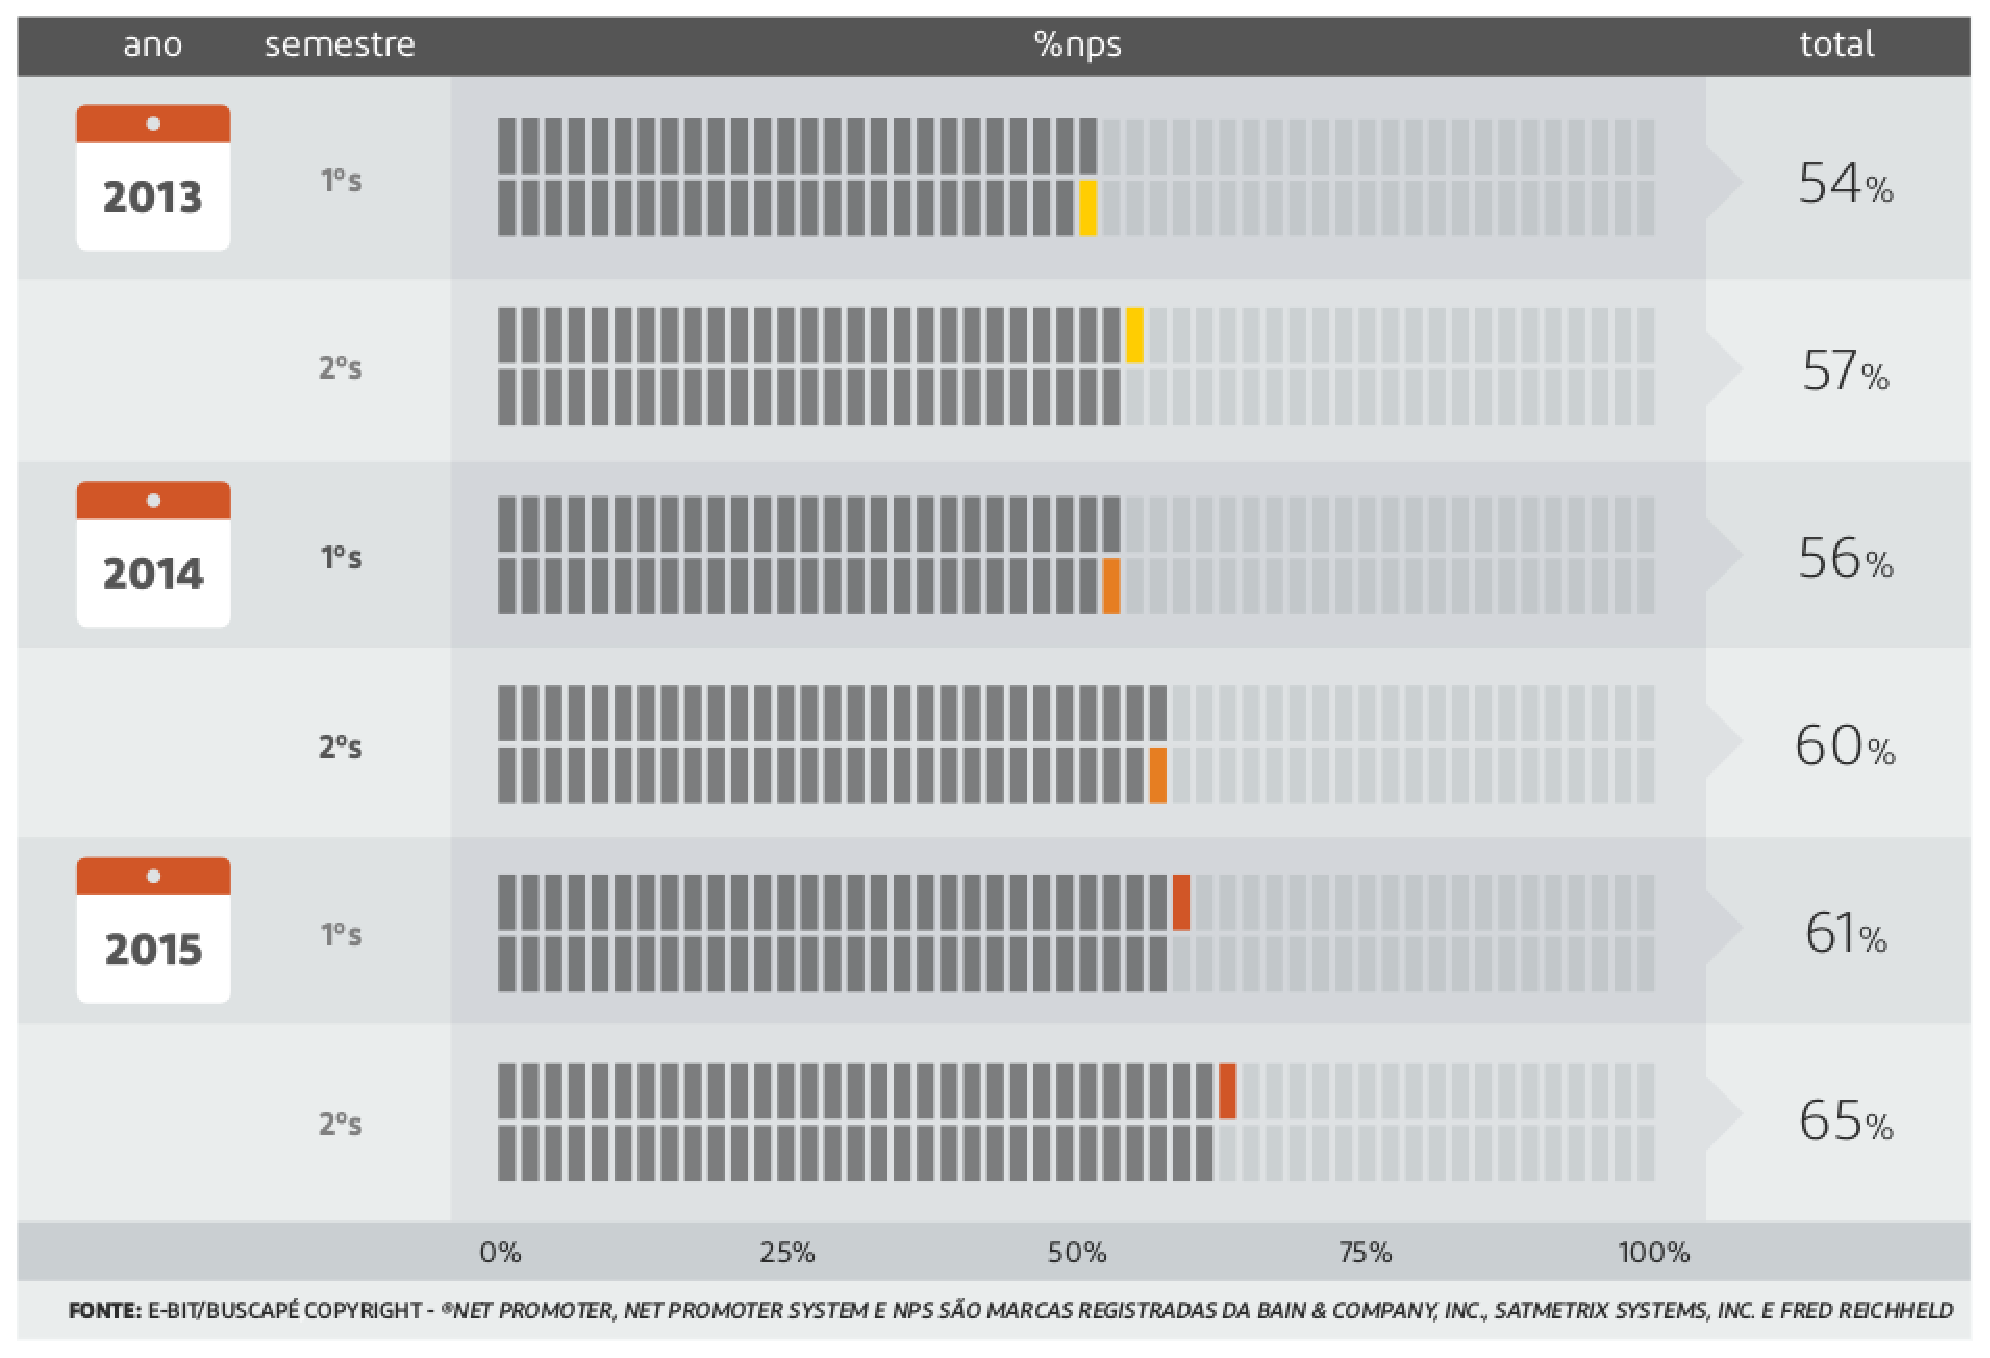
\includegraphics[width=12cm]{img/webshoppers/nps.eps}
\caption{Satisfação e fidelização de clientes}
\small{Fonte: \citeonline{webshoppers} - Relatório WebShoppers}
\label{figura:nps}
\end{figure}

Vitor Augusto Meira França, economista da Fecomercio-SP principal entidade sindical paulista dos setores de comércio e serviços. Responsável por administrar, no Estado, o Serviço Social do Comércio (Sesc) e o Serviço Nacional de Aprendizagem Comercial (Senac) afirma o seguinte:

\begin{citacao}
Diante de um quadro de instabilidade política, inflação alta, taxas de juros elevadas, escassez de crédito, aumento do desemprego e consequente conservadorismo dos consumidores, o varejo brasileiro deve repetir o fraco desempenho do ano passado e registrar nova queda das vendas neste ano. por outrolado, o e-commerce deve apresentar crescimento como ocorreu em 2015. \cite{webshoppers}
\end{citacao}

A figura \ref{figura:estimativa:faturamento} apresenta estimativas relacionadas ao faturamento do \textif{e-commerce}, para o ano de 2016, no Brasil.

\begin{figure}[H]
\centering
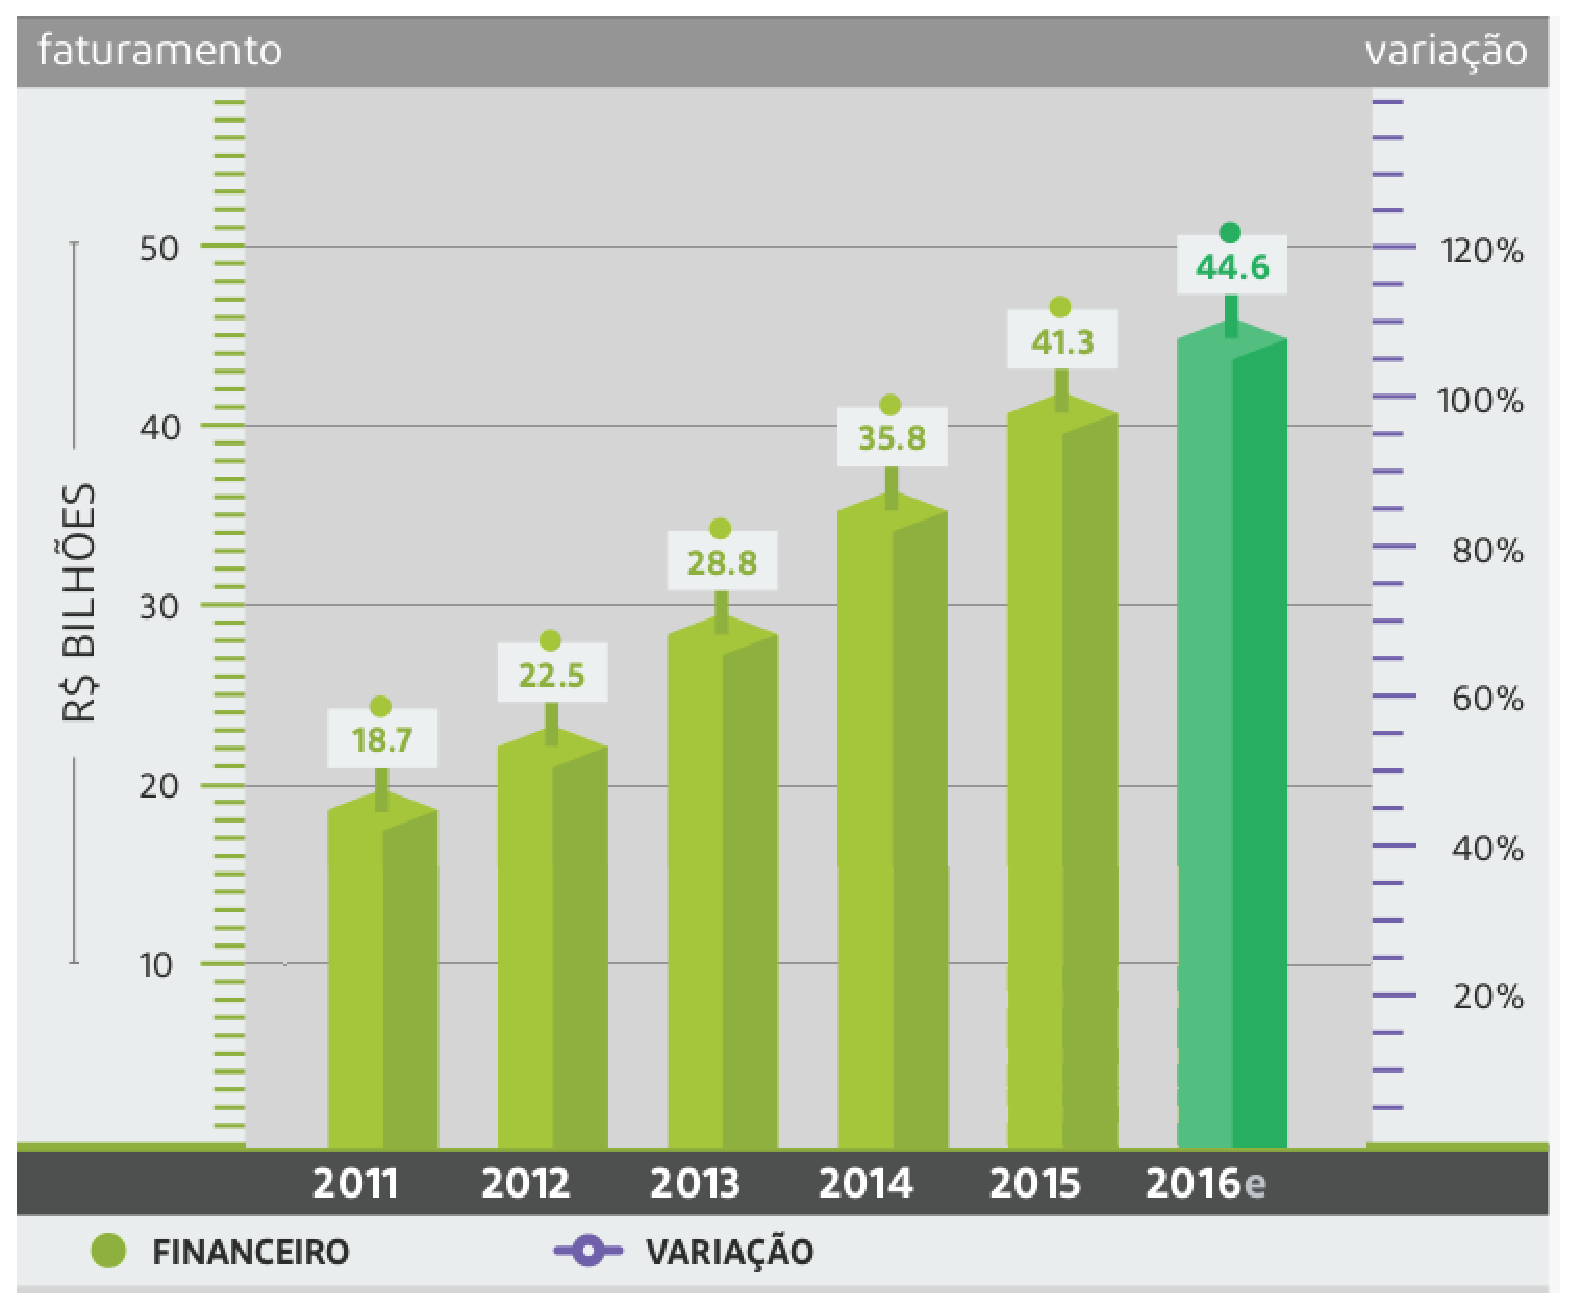
\includegraphics[width=12cm]{img/webshoppers/estimativa-faturamento.eps}
\caption{Estimativa de faturamento do \textit{e-commerce} para 2016}
\small{Fonte: \citeonline{webshoppers} - Relatório WebShoppers}
\label{figura:estimativa:faturamento}
\end{figure}

Diante esses dados sobre o \textit{e-commerce} no brasil, percebe-se que o comércio eletrônico é um mercado em ascenção.

Entre os empresários que se aventuram nesse ambiente, um dos anseios é ter uma loja que tenha a identidade visual da sua marca, que possibilite formas práticas e seguras de compra pelos clientes e, claro, que seja de fácil manuseio e administração para ele mesmo. Com ferramentas como o Mercado Livre\footnote{https//www.mercadolivre.com.br}, por exemplo, é possível disponibilizar produtos para a venda, mas em um ambiente diferente de uma loja virtual particular.
% chapter introdução(end)

\section{Motivação} % (fold)
\label{sec:motivacao}

Existem muitas ferramentas que facilitam a criação e gestão de lojas virtuais, porém algumas delas não são populares e as vezes desconhecidas, tais ferramentas poderiam ajudar a expandir um negócio ou criar uma oportunidade para aqueles que desejam empreeder através de vendas na Internet. 

Segundo \citeonline{felipini}, ``Um e-commerce pode ser implantado aos poucos e testado''. Diferentemente de uma empresa tradicional, em que o início das operações ocorre somente com o empreendimento totalmente estruturado, um negócio na Internet pode ser implantado em etapas, o que dilui o investimento e facilita a correção de erros. Por exemplo, um estabelecimento de vendas só receberá seu primeiro cliente após a loja estiver totalmente pronta. Na Internet, você pode montar um site de conteúdo, com ou sem sua marca definitiva, testar a aceitabilidade de seu modelo de negócio e produtos, avaliar a visitação e, somente depois, começar a vender. Dessa forma, mesmo aqueles que ainda não possuam um negócio, poderão investir em um \textit{e-commerce}.

Os comerciantes já fixados no mercado e interessados em colocar seu negócio na rede, procuram por empresas especializadas em desenvolvimento de softwares para desenvolver seu site de vendas. O problema nisso é que o custo pode ser alto. \citeonline{jalote} afirma: ``O software é caro porque torna se uma atividade difícil e trabalhosa de ser realizado pelo engenheiro de software''.  Outro problema realacionado ao desenvolvimento de software no geral, isso inclui uma loja virtual, é o tempo. O que gera insatisfação dos clientes, pela demora no cumprimento dos prazos \cite{pressman}.

Além desses, um outro problema é a manutenção do site. Segundo \citeonline{sommervile} manutenção de software é a modificação de um programa após ter sido colocado em uso. Mundanças por exemplo, em alterar o \textit{layout}\footnote{Aspecto visual das páginas do site} geram custos e podem também ser demoradas.

A Sudo Loja, visa resolver esses problemas oferecendo um CMS (do inglês \textit{Content Management System}), capaz de criar, gerenciar e tornar possível a personalização de uma loja virtual. O CMS proposto busca facilitar a criação e gestão de um \textit{e-commerce}, promovendo uma entrada rápida ao mercado virtual à pequenas e médias empresas. Podem ser vistos vários sistemas que funcionam dessa maneira, como por exemplo: a \citeonline{tray} e \citeonline{lojaintegrada}. Na Seção \ref{cha:ferramentas_relacionadas} será apresentado um comparativo entre estas e outras ferramentas.


% section motivacao (end)

\section{Objetivos} % (fold)
\label{sec:objetivos}

Esta seção apresenta os objetivos que direcionarão a construção do sistema.

\subsection{Objetivo Geral} % (fold)
\label{sub:objetivo_geral}

Esse trabalho tem como objetivo principal o desenvolvimento de uma ferramenta para criação de lojas virtuais, onde um usuário cadastrado poderá criar um ou mais lojas, personalizar seu \textit{layout} e disponibilizar produtos para a venda.

% subsection objetivo_geral (end)

\subsection{Objetivos Específicos} % (fold)
\label{sub:objetivos_espec}

\begin{itemize}
\item Prover uma alternativa de \textit{e-commerce} para a região.
\item Tornar acessível financeiramente, manter seu próprio \textit{e-commerce}.
\item Incentivar o uso de novas soluções em TI nas pequenas e médias empresas comerciais da região.
\item Facilitar a entrada de novos comerciantes no mercado virtual.
\item Quanto a ferramenta, desenvolver um painel administrativo para que os usuários possam acompanhar e gerenciar sua loja.
\item Tornar possível a criação de mais de uma loja com a mesma conta de usuário.
\item Disponibilizar um módulo para personalização das lojas.
\end{itemize}
% subsection objetivos_espec (end)

% section objetivos (end)

\section{Organização do Documento} % (fold)
\label{sec:organizacao_do_documento}

% section organizacao_do_documento (end)
A Seção \ref{cha:fundamentaco_teorica} apresenta a fundamentação teórica para o desenvolvimento deste trabalho. Na Seção \ref{cha:metodologia} é descrita a metodologia adotada para execução do projeto. A Seção \ref{cha:sudoloja} descreve a solução proposta no trabalho, um comparativo entre ferramentas do gênero e também as etapas de análise, projeto, implementação e validação do sistema. A Seção \ref{cha:consideracoes_finais} apresenta as considerações finais do trabalho, assim como discuções sobre trabalhos futuros. Por fim, os artefatos gerados no decorrer do desenvolvimento do trabalho podem ser vistos nos Apêndices.

\chapter{Fundamentação Teórica} % (fold)
\label{cha:fundamentaco_teorica}

Essa seção discutirá sobre alguns assuntos necessários para obter um melhor entendimento do trabalho.

\section{CMS} % (fold)
\label{sec:cms}

Sistemas de Gerenciamento de Conteúdo (SGC) ou Content Management System (CMS), segundo \citeonline{mercer} são softwares que facilitam a criação, organização, manipulação e remoção de dados em forma de imagens, documentos, scripts, textos, etc.
Já \citeonline{barcia}, diz que um CMS, é uma plataforma de gestão de conteúdos, ou seja, um sistema que integra ferramentas que permitem criar, editar e publicar conteúdo em tempo real, onde os utilizadores manipulam uma interface sem terem a necessidade de saber programar. \citeonline{barcia} ainda ressalta que os gerenciadores também dispensam o uso de programação, facilitando dessa forma a gestão dos dados e o acesso às funcionalidades da ferramenta.

O uso de um CMS pode facilitar o trabalho dos administradores de aplicações, que envolvem muitas atualizações no seu conteúdo, como por exemplo, blogs, portais corporativos\footnote{Instrumento de gestão de informação e de conhecimento}. ``Os benefícios ligados a adoção de um CMS incluem desde a redução do custo de atualização dos conteúdos nos websites até o aumento da eficiência das equipes de TI'' \cite{pereira}.

Em linhas gerais, um CMS permitiria administrar conteúdos em meio digital. E para o caso particular que nos ocupa, um CMS permitiria gerenciar os conteúdos de uma loja virtual.

Em outras palavras, um CMS é uma ferramenta que permite a um editor criar e publicar qualquer tipo de informação em uma página web. Geralmente, um CMS trabalha manipulando um banco de dados, de modo que o editor simplesmente atualiza este banco, incluindo nova informação ou editando a existente.

Contudo, o mais interessante, é que essa ferramenta é feita de tal maneira que mesmo aqueles que nunca ouviram falar de JAVA, PHP, MySQL, Javascript ou qualquer outra linguagem voltada para web poderá usá-lo, inclusive esta é sua principal função, tornar acessível a todos a sua presença na Internet através de um site, facilitando a inserção de textos, de comentários e dezenas de outras funcionalidades, de acordo com as características de cada aplicação. Alguns Exemplos de CMS podem ser vistos a seguir.

\begin{itemize}
\item \textit{Drupal} - É uma plataforma de gerenciamento de conteúdo de código aberto, usado em milhares de web sites e aplicações. Ele é desenvoldivo, usado, e apoiado por uma comunidade ativa e diversificada de pessoas ao redor do mundo \cite{drupal}.

\item \textit{OpenText} \citeyear{opentext} - O primeiro sistema CMS comercial que apareceu no mercado. A OpenText é líder em Gestão de Informação Corporativa. Seus produtos de gerenciamento de conteúdo permitem uma coleta mais eficiente de todos os tipos de informação - estruturada e não estruturada - e fornecem essa informação em contexto por qualquer aplicativo, plataforma ou processo \cite{opentext}.

\item \textit{Wordpress} - Sistema muito popular e bastante usado pelos \textit{bloggers}. WordPress é um software web que você pode usar para criar um site, blog, ou app \cite{wordpress}.
\end{itemize}

% section cms (end)

\section{\textit{E-commerce}} % (fold)
\label{sec:e_commerce} 

Segundo \citeonline{kalakota}, o Comércio Eletrônico (CE) pode ser definido como sendo a compra e a venda de informações, produtos e serviços através de redes de computadores. \citeonline{bloch} estenderam esta definição incluindo que CE é o suporte para qualquer tipo de transações de negócio sobre uma infra-estrutura digital.

\apudonline{kalakota}{albertin} há muito tempo, consideravam que o ambiente tradicional de negócio estava mudando rapidamente, com os consumidores e negócios procurando flexibilidade para mudar os parceiros de negócio, plataformas, carreiras e redes. O \textit{e-commerce} começava a se disseminar.

O comércio eletrônico ou \textit{e-commerce}, é aplicável a qualquer tipo de transação comercial que pode envolver compra, venda, transferência ou troca de produtos, serviços ou informações por meio de redes de computadores, incluindo a Internet \cite{turban}.

Existem diferenças entre \textit{e-commerce} e \textit{e-business}. \textit{E-business} é definido como o uso das tecnologias da informação para executar funções de negócios. \textit{E-business} é, portanto, um termo mais amplo que inclui \textit{e-commerce} \cite{gordon}. 

Dentre os modelos existentes de \textit{e-business}, \citeonline{asfoura} destacam três tipos principais que incluem o e-commerce em sua execução:

\begin{itemize}
\item \textbf{Empresa para Empresa (B2B – Business to Business):} Engloba as negociações de bens ou serviços que acontecem entre empresas;
\item \textbf{Empresa para Consumidor (B2C – Business to Consumer):} Tipo de comércio mais conhecido, onde a empresa faz o negócio diretamente com os consumidores finais;
\item \textbf{Consumidor para Consumidor (C2C – Consumer to Consumer):} Engloba todas as transações que acontecem entre consumidores finais, geralmente intermediadas por uma terceira entidade;
\end{itemize}

O sistema que será apresentado se encaixa no modelo de negócio B2C (\textit{Business to Consumer}), onde o lojista fará o negócio diretamente com os consumidores finais.

\section{YP} % (fold)
\label{sec:yp}

Quando se trabalha na elaboração de um produto os sistema, é importante seguir uma série de passos previsíveis - um roteiro que ajude a criar um resultado de alta qualidade e dentro de prazo estabelecido. O roteiro é denominado ``Processo de Software'' \cite{pressman}.

O \textit{easyProcess}, comumente chamado de YP. É um processo de \texit{software} criado com o objetivo de sanar as dificuldades dos alunos em se adaptar aos processos já existentes para o uso na academia. Voltado a projetos de pequeno escopo, o YP foca-se na aprendizagem do processo com alguns elementos qualificadores: uma boa produtividade, bom uso do ferramental de apoio e geração mínima de artefatos, além de se buscar uma consolidação do entendimento das práticas e conceitos da Engenharia de Software \cite{easyprocess}. O fluxo básico do YP está ilustrado na figura \ref{figura:yp}.

\begin{figure}[H]	
\centering
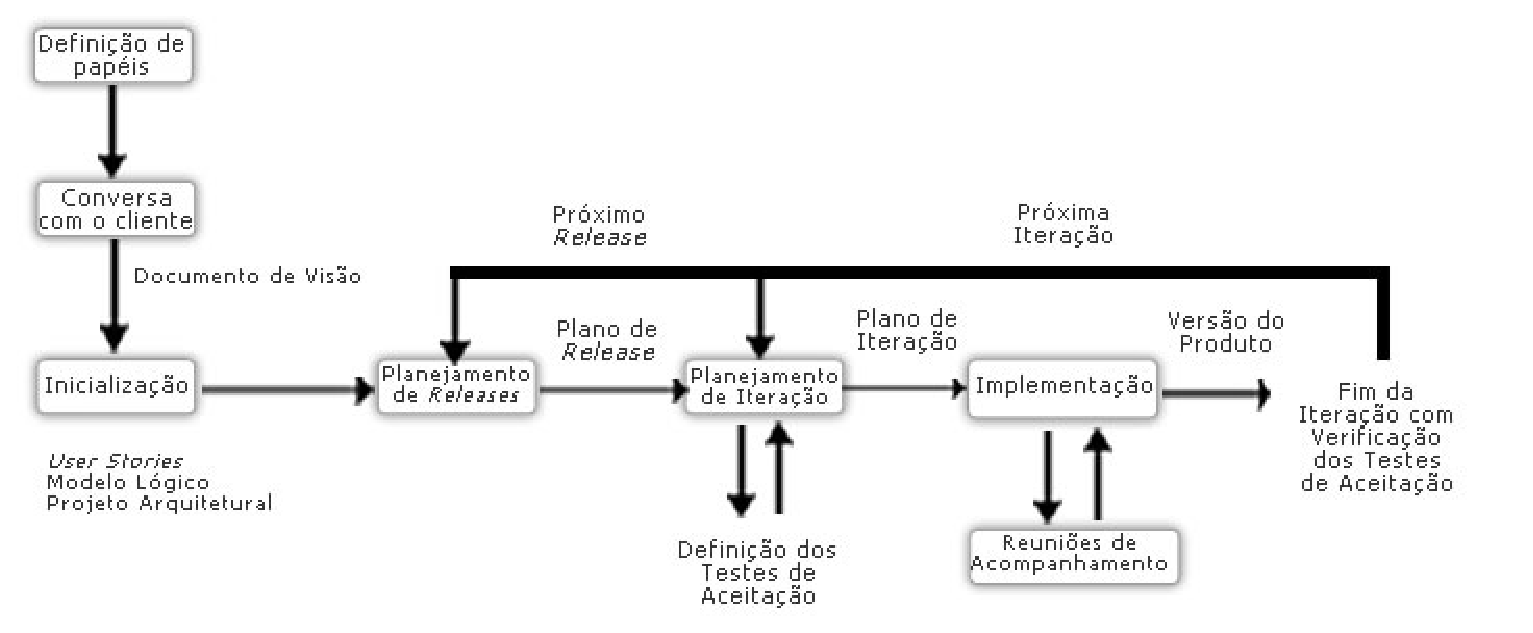
\includegraphics[width=15cm]{img/yp.eps}
\caption{Fluxo do \textit{easyProcess}}
\label{figura:yp}
\end{figure}

A primeira etapa do processo consiste na \textbf{Definição de papéis}. Em seguida deve ser realizada uma \textbf{Conversa com o cliente}. Na fase de \textbf{Inicialização} o cliente define as \textit{User Stories}\footnote{Funções que o sistema deve desempenhar e que são definidas pelo cliente e pelo desenvolvedor} e são elaborados o projeto arquitetural e o modelo lógico de dados, este último apenas se necessário. Parte-se então para o \textbf{Planejamento} e em seguida para a \textbf{Implementação}. O andamento do processo deve ser coordenado pelo gerente através da \textbf{Reunião de Acompanhamento} semanal que visa recolher e analisar métricas.

% section yp (end)

% section e_commerce (end)
% chapter fundamenta_o_te_rica (end)

\chapter{Metodologia} % (fold)
\label{cha:metodologia}

A realização dos estudos deste trabalho segue a mesma metodologia de trabalhos científicos. "Ciêntifico não é considerado como algo pronto, acabado ou definitivo” \cite{sa2010anuario}, isso permite que os contextos existentes sejam interpretados e discutidos de diferentes formas por diferentes pessoas.

Métodos científicos são as formas mais seguras inventada pelo homem para controlar o movimento das coisas que cerceiam um fato e montar formas de compreensão adequadas de fenômenos \cite{bunge}.

Abaixo está descrita a metodologia seguida para o desenvolvimento deste trabalho:

\begin{itemize}
	\item \textbf{Determinação do tema} - Nesta fase, foi verificada o tema foco do trabalho, o qual foi posteriormente avaliado por membros do corpo docente da instituição.

	\item \textbf{Levantamento bibliográfico} - Com o tema estabalecido, foi efetuado um estudo bibliográfico, afim de fundamentar o tema.

	\item \textbf{Leitura e Documentação} - Foi de competência desta fase, a filtragem e entendimento do material encontrado conforme a relevância da publicação;

	\item \textbf{Construção lógica} - As ideias da pesquisa foram estruturadas conforme as exigências racionais da sistematização própria do trabalho.

	\item \textbf{Construção do texto e articulação dos parágrafos} - O desenvolvimento do texto foi organizado em capítulos, cada qual abordando diferentes ênfases.

	\item \textbf{Projeto e desenvolvimento} - Fase prática da exploração das referências bibliográficas, para esta etapa o uso do processo de desenvolvimento YP foi adotado e é descrito em detalhes na seção \ref{sec:processo_de_desenvolvimento}.

	\item \textbf{Conclusão} - Terminado as fases anteriores, a conclusão define o resultado obtido, a aplicabilidade da Sudo Loja e discussões sobre trabalhos futuros.
\end{itemize}

\section{Processo de desenvolvimento} % (fold)
\label{sec:processo_de_desenvolvimento}

Esta seção abordará em detalhes como se deu a utilização do processo \textit{easYProcess} no desenvolvimento do sistema.

\section{Atividades} % (fold)
\label{sec:atividades}

Nesta seção serão abordadas as atividades realizadas durante o processo de desenvolvimento do sistema, seguindo as diretrizes do \textit{easYProcess}, estas são: Definição de papéis, na Subseção \ref{sub:definicao_de_papeis}; Conversa com o Cliente, na Subseção \ref{sub:conversa_com_o_cliente}; Inicialização, na Subseção \ref{sub:inicializacao}; E Planejamento de \textit{Releases}, na Subseção \ref{sub:planejamento_de_releases}.

\subsection{Definição de Papéis} % (fold)
\label{sub:definicao_de_papeis}

Após a etapa de definição de Papéis chegamos ao seguinte resultado, que pode ser visto no Quadro \ref{quadro:papeis}:

\begin{table}[H]
\centering
\caption{Definição de Papéis}
\label{quadro:papeis}
\begin{tabular}{|a|b|}
\rowcolor{ballblue}
\hline
\textbf{Papel} & \textbf{Stakeholder}\\
\hline
Cliente  	   & Francisco Paulo de Freitas Neto\\
\hline
Usuário  	   & Francisco Paulo de Freitas Neto\\
\hline
Testador 	   & João Marcos Ferreira\\
\hline
Desenvolvedor & João Marcos Ferreira\\
\hline
Gerente 	   & João Marcos Ferreira\\
\hline 
\end{tabular}
\end{table}


% section defini_es_de_pap_is (end)

\subsection{Conversa Com o Cliente} % (fold)
\label{sub:conversa_com_o_cliente}
Aqui são onde informações sobre o escopo do problema são adquiridas. A partir de então, a equipe encontra-se apta a gerar o documento de visão, que após ser validado pelo cliente, funciona como um acordo de trabalho entre cliente e equipe de desenvolvimento. O Documento de visão produzido durante esta etapa pode ser visto no Apêndice \ref{ap:documento_visao} Documento de Visão.

% subsection conversa_com_o_cliente (end)

\subsection{Inicialização} % (fold)
\label{sub:inicializacao}
Como sugerido pelo YP, nesta fase foram definidas as \textit{Users Stories} e suas respectivas estimativas de tempo para implementação.  Com isso pôde-se verificar a viabilidade de desenvolvimento do projeto no escopo e tempo definidos. As \textit{Users Stories} capturadas podem ser vistas a seguir no quadro \ref{quadro:userstories}. Nas seções seguintes uma delas será apresentada com detalhes e as demais poderão ser vistas no Apêndice \ref{app:user_stories_e_testes_de_aceitacao} \textit{\textit{User Stories}} e Testes de Aceitação.	

\begin{longtable}{|p{3cm}|p{9cm}|p{3cm}|}
\caption{\textit{\textit{User Stories}} levantadas}
\label{quadro:userstories}
\hline
\rowcolor{ballblue}
\textbf{Identificação} & \textbf{Descrição} & \textbf{Estimativa}\\
\hline
\textbf{US01} & O sistema deve realizar o gerenciamento dos perfis de clientes logistas. & 1 semana.\\
\hline
\textbf{US02} & O sistema deve realizar o gerenciamento dos dados das lojas virtuais. & 1 semana.\\
\hline
\textbf{US03} & O sistema deve realizar o gerenciamento do estoque da loja virtual. & 2 semanas.\\
\hline
\textbf{US04} & O sistema deve disponibilizar uma página de gerenciamento para os clientes logistas. & 2 semanas.\\
\hline
\textbf{US05} & O sistema deve permitir a personalização do Layout da página da sua loja virtual. & 3 semanas.\\
\hline
\textbf{US06} & O sistema deve realizar o gerenciamento dos perfis de clientes da loja virtual. & 1 semana.\\
\hline
\textbf{US07} & O sistema deve disponibilizar uma página de acompanhamento para os clientes. & 1 semana.\\
\hline
\textbf{US08} & Nas páginas dos produtos deve ser possível realizar perguntas ao vendedor. & 1 semana.\\
\hline
\textbf{US09} & O sistema deve calcular o frete dos produtos automaticamente. & 3 dias.\\
\hline
\textbf{US10} & As páginas dos produtos deve apresentar uma galeria imagens por produto. & 3 dias.\\
\hline
\textbf{US11} & O sistema deve concretizar vendas através de diferentes meios de pagamento. & 1 semana.\\
\hline
\end{longtable}	

Também foi elaborado o modelo lógico de dados da aplicação que pode ser visto na figura \ref{figura:modelo_logico}. Algumas entidades do modelo lógico apresentado a seguir, não foram documentadas por não estarem completamente definidas no projeto de TCC1. No documento de TCC2 poderá ser visto um modelo que contemplará o sistema como um todo.

\begin{figure}[H]
\centering
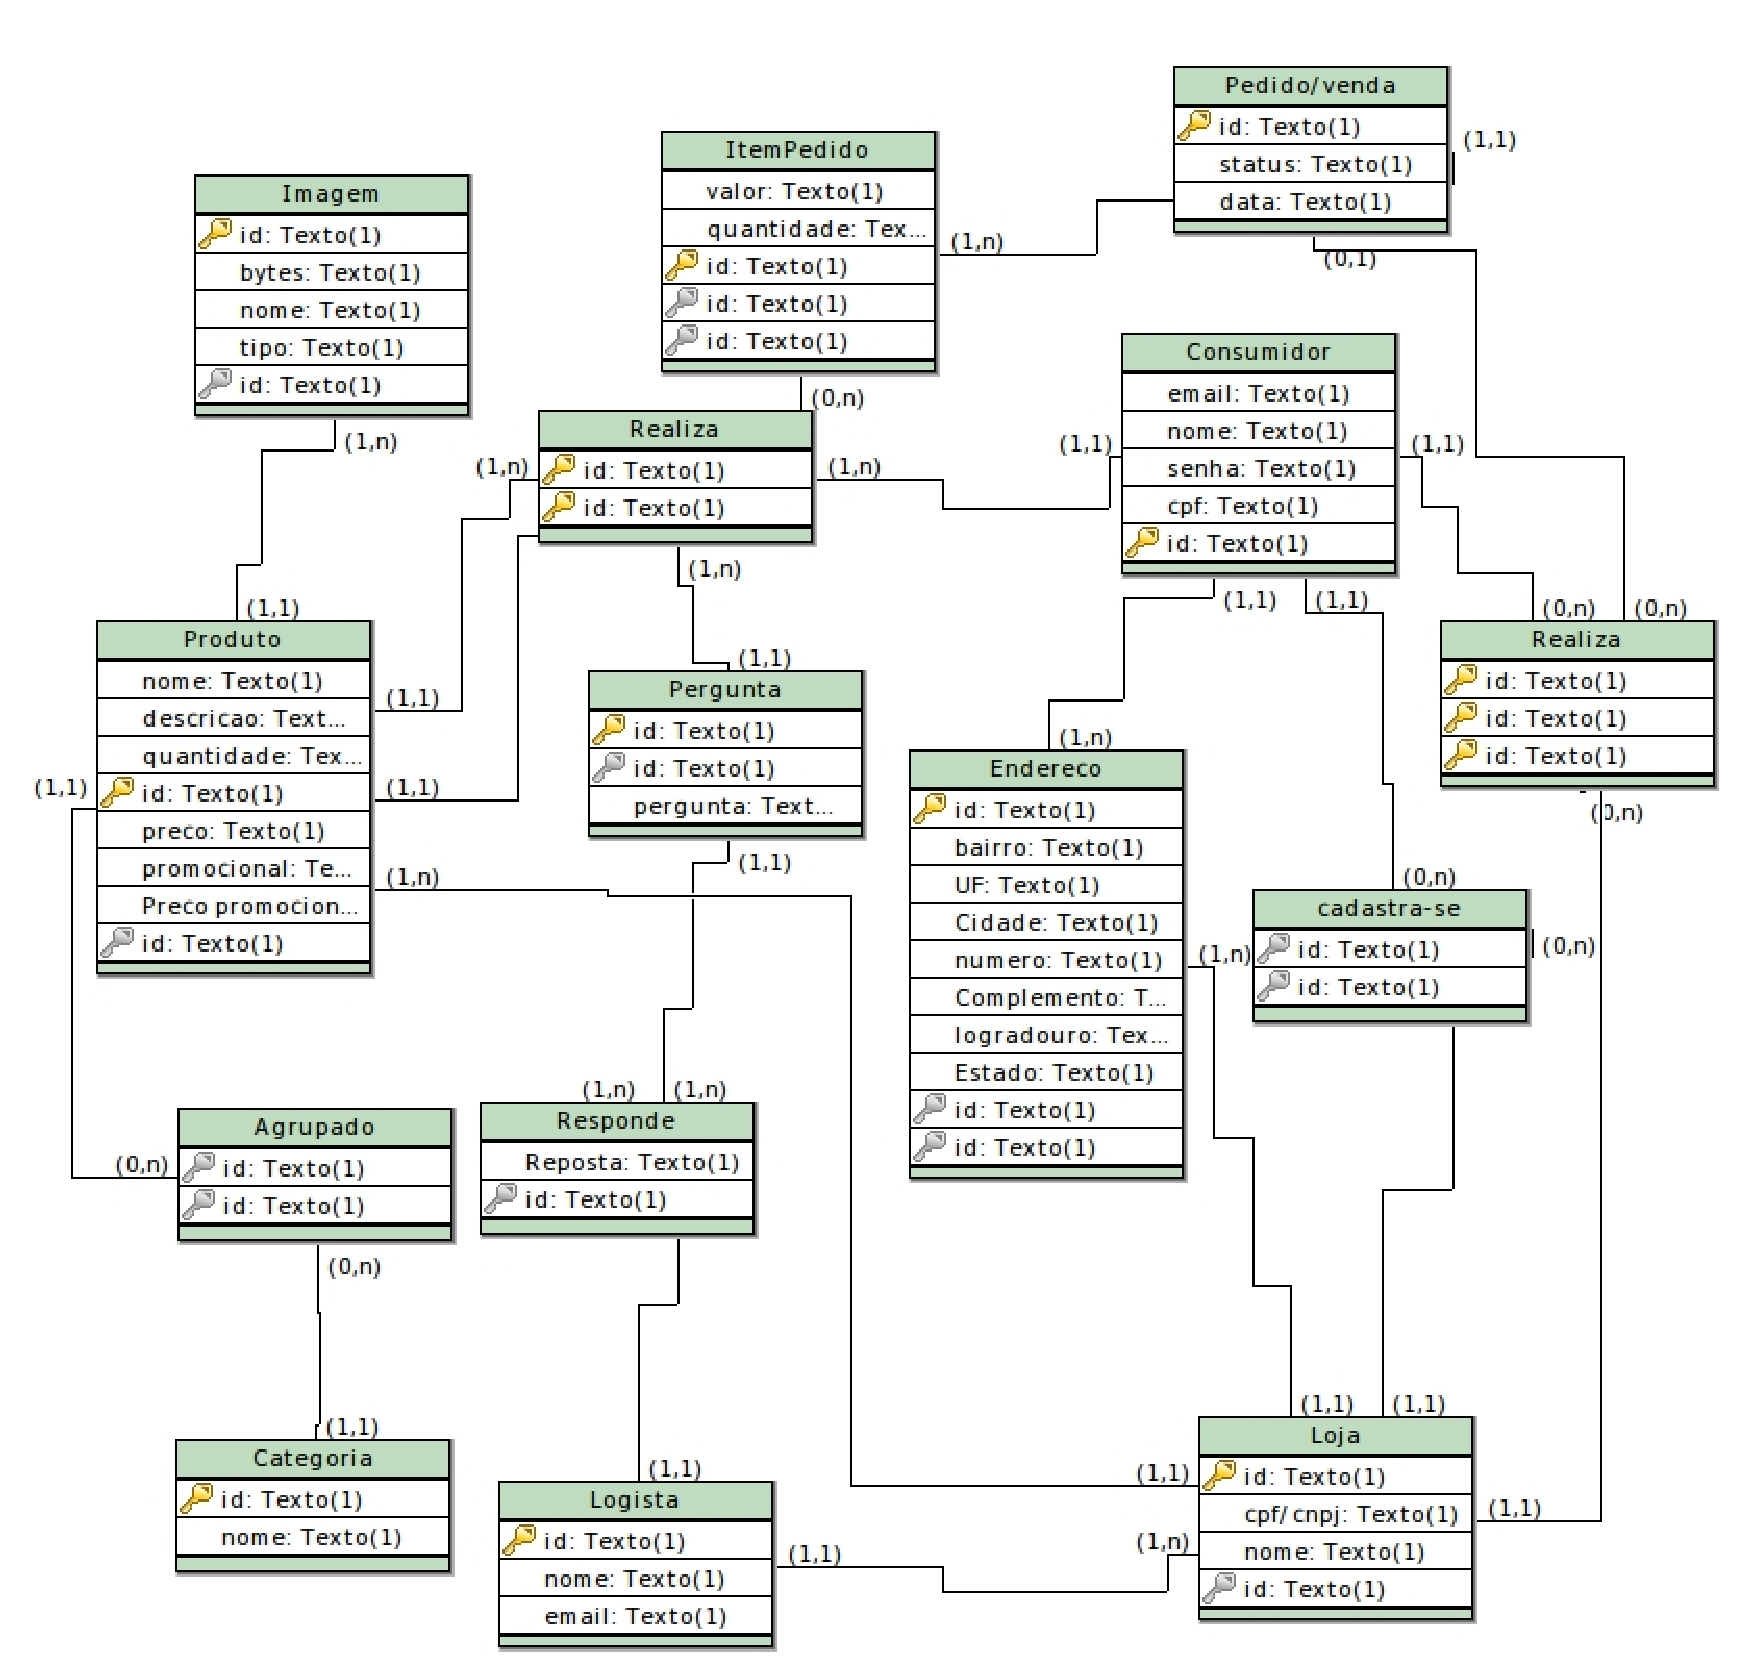
\includegraphics[width=15cm]{img/modelo_logico.eps}
\caption{Modelo logico de Dados}
\label{figura:modelo_logico}
\end{figure}

\subsection{Planejamento de Releases} % (fold)
\label{sub:planejamento_de_releases}

Durante esta etapa foram definidas as \textit{Releases}, juntamente com a data estimada para o termino de seu desenvolvimento. Esses dados podem ser vistos no apendice \ref{apdc:plano_de_itercao} Plano de Iteração.

% subsection planejamento_de_releases (end)

% section atividades (end)
% section processo_de_desenvolvimento (end)

% chapter metodologia (end)


% \chapter{Sudo Loja} % (fold)
% \label{cha:sudo_loja}

% Esta seção irá discutir o sistema desenvolvido, assim como as etapas de análise, projeto e implementação. Também será abordado o projeto arquitetural e as tecnologias utilizadas na construção do sistema. Na seção \ref{sec:ferramentas_relacionadas} uma análise das ferramentas relacionadas foi levantada, afim de destacar um diferencial dentre as ferramentas existentes.

% \section{Ferramentas Relacionadas} % (fold)
% \label{sec:ferramentas_relacionadas}

% A seguir, podemos ver um quadro comparativo com as principais ferramentas usadas na criação de lojas virtuais e suas respectivas funcionalidades comparando com o sistema desenvolvido.

% \begin{itemize}
% \item 1. Magento (www.magento.com) \nocite{magento}
% \item 2. Tray Commerce (www.tray.com.br) \nocite{tray}
% \item 3. Loja UolHost (www.uolhost.com.br) \nocite{uolhost}
% \item 4. Wix Commerce (pt.wix.com/ecommerce/website) \nocite{wix}
% \item 5. Loja Integrada (www.lojaintegrada.com.br) \nocite{lojaintegrada}

% \end{itemize}

% \begin{table}[H]
% \centering
% \caption{Funcionalidades das ferramentas}
% \label{quad:comparativo}
% \begin{tabular*}{\textwidth}{@{\extracolsep{\fill}} |a|b|b|b|b|b|b|}	
% \hline
% \rowcolor{ballblue}
% & 1 	  & 2 	          & 3 			 & 4 			& 5   & Sudo Loja\\ 
% \hline
% Pago										 	& não     & sim			  & sim			 & sim 			& sim & \textbf{não}\\
% \hline
% Gerenciamento de produtos, 			& sim     & sim			  & sim			 & sim 			& sim & \textbf{sim}\\
% clientes e pedidos 			&      & 			  & 			 &  			&  & \\
% \hline
% Personalização do layout 					 	& sim     & sim			  & sim			 & sim 			& sim & \textbf{sim}\\
% \hline
% Múltiplas imagens por produto 				 	& sim     & sim			  & sim			 & sim 			& sim & \textbf{sim}\\
% \hline
% Site apropriado para dispositivos moveis    	& sim     & não			  & não			 & não 			& não & \textbf{sim}\\
% \hline
% Controle de estoque								& sim     & sim			  & sim			 & sim 			& sim & \textbf{sim}\\
% \hline
% Perguntas na página do produto 			& não     & não			  & não			 & não 			& não & \textbf{sim}\\
% \hline
% \end{tabular*}
% \end{table}

% Como o quadro \ref{quad:comparativo} mostra, a Sudo Loja contará com as funcionalidades encontradas nas ferramentas listadas acima e ainda com um diferencial, que será a possibilidade de fazer perguntas ao vendedor sobre determinado produto.

% % section ferramentas_relacionadas (end)

% \section{Análise} % (fold)
% \label{sec:analise}

% A seguir serão apresentados os artefatos produzidos na fase de análise, inerentes a uma \textit{User Story} específica. Para isso foi escolhida a \textit{User Story} 03 (O sistema deve realizar o gerenciamento do estoque da loja virtual).

% As \textit{User Stories} alocadas são quebradas em tarefas, e o cliente deve definir os testes de aceitação para cada \textit{User Story}. Para auxílio na gerência foi feito uso da Tabela de Alocação de Tarefas (TAT), na qual especificamos as \textit{\textit{User Stories}} envolvidas, tarefas, responsáveis, estimativas de tempo, tempo real consumido e status da tarefa. Nos quadros \ref{quadro:tati-us03} e \ref{quadro:teste-aceitacaoi-us03} podemos ver, respectivamente, a tabela de alocação de tarefas e os testes de aceitação geradas pra a US03. As demais \textit{\textit{User Stories}} serão apresentadas com detalhes no Apêndice \ref{app:user_stories_e_testes_de_aceitacao}.

% \newpage

% \begin{longtable}{|p{1.5cm}|p{3.5cm}|c|p{2cm}|p{2cm}|c|}
% \caption{Alocação de Tarefas - US03}
% \label{quadro:tati-us03}
% \hline
% \multicolumn{6}{|c|}{\textbf{\textit{User Story} 03}}\\
% \hline		
% \rowcolor{ballblue}
% Tarefa & Descrição & Responsável & Estimativa de tempo (horas) & Tempo real (horas) & Status\\
% \hline
% T1 & Implementar Script para salvar um Produto & João Marcos & 2 & 1 & Finalizado\\
% \hline
% T2 & Implementar Script para validar informações do produto & João Marcos & 2 & 1 & Finalizado\\
% \hline
% T3 & Criar Formulário para cadastro de produto & João Marcos & 3 & 2 & Finalizado\\
% \hline
% T4 & Criar formulário para edição de produto & João Marcos & 2 & 1 & Finalizado\\
% \hline
% T5 & Criar página para o estoque, exibindo as informações básicas de cada produto com sua respectiva quantidade e link para ficha do produto & João Marcos & 4 & 3 & Finalizado\\
% \hline
% T6 & Criar botão para exclusão de um produto na página de estoque & João Marcos & 2 & 1 & Finalizado\\
% \hline
% \end{longtable}

% \begin{longtable}{|l|p{11.8cm}|c|}
% \caption{Teste de aceitação - US03}
% \label{quadro:teste-aceitacaoi-us03}
% \hline
% \multicolumn{3}{|c|}{\textbf{\textit{User Story} 03}}\\
% \hline		
% \rowcolor{ballblue}
% \multicolumn{2}{|c|}{Testes de aceitação} & Status\\	
% \hline
% TA1 & Dado que estou na página de cadastro de produto, quando eu preencher o formulário com os dados obrigatórios de forma correta , o produto deve ser salvo e informado uma mensagem de sucesso.   & Finalizado\\
% \hline
% TA2 & Dado que estou na página de cadastro de produto, quando eu preencher o formulário com os dados obrigatórios de forma incorreta , o produto não deve ser salvo e uma mensagem de erro deve ser exibida.   & Finalizado\\
% \hline
% TA3 & Dado que estou acessando a ficha de edição de produto, quando eu alterar alguma informação do formulário com os dados válidos, o produto deve ser atualizado e uma mensagem de sucesso deve ser exibida.   & Finalizado\\
% \hline
% TA4 & Dado que estou acessando a ficha de edição de produto, quando eu alterar alguma informação do formulário com os dados inválidos, tais informações não serão salvas e uma mensagem de erro deve ser exibida.   & Finalizado\\
% \hline
% TA5 & Dado que estou na página de estoque, quando eu selecionar a opção excluir este produto, um diálogo de confirmação deve ser exibido. Caso confirme o produto deve ser excluído  & Finalizado\\
% \hline
% TA6 & Dado que estou na página de estoque, quando eu selecionar a opção excluir este produto, um diálogo de confirmação deve ser exibido. Caso não confirme o produto não deve ser excluído  & Finalizado\\
% \hline
% \end{longtable}

% % section analise (end)

% \section{Projeto Arquitetural} % (fold)
% \label{sec:projeto_arquitetural}

% O sistema será organizado em 3 camadas, são elas: Apresentação, Serviços e Persistência. As próximas seções abordarão individualmente cada uma delas. Segundo \citeonline{sommerville}, o modelo em camadas de uma arquitetura organiza o sistema em camadas, cada uma das quais fornecendo um conjunto de serviços, essa abordagem apoia o desenvolvimento incremental de sistemas. À medida que uma camada é desenvolvida, alguns serviços disponibilizados por essa camada podem ser disponibilizadas para os usuários. Na Figura \ref{fig:representacao-pa}, pode ser vista uma representação visual de como se dará a organização das camadas, onde cada camada só acessa diretamente suas camadas adjacentes.

% \begin{figure}[H]
% \centering
% 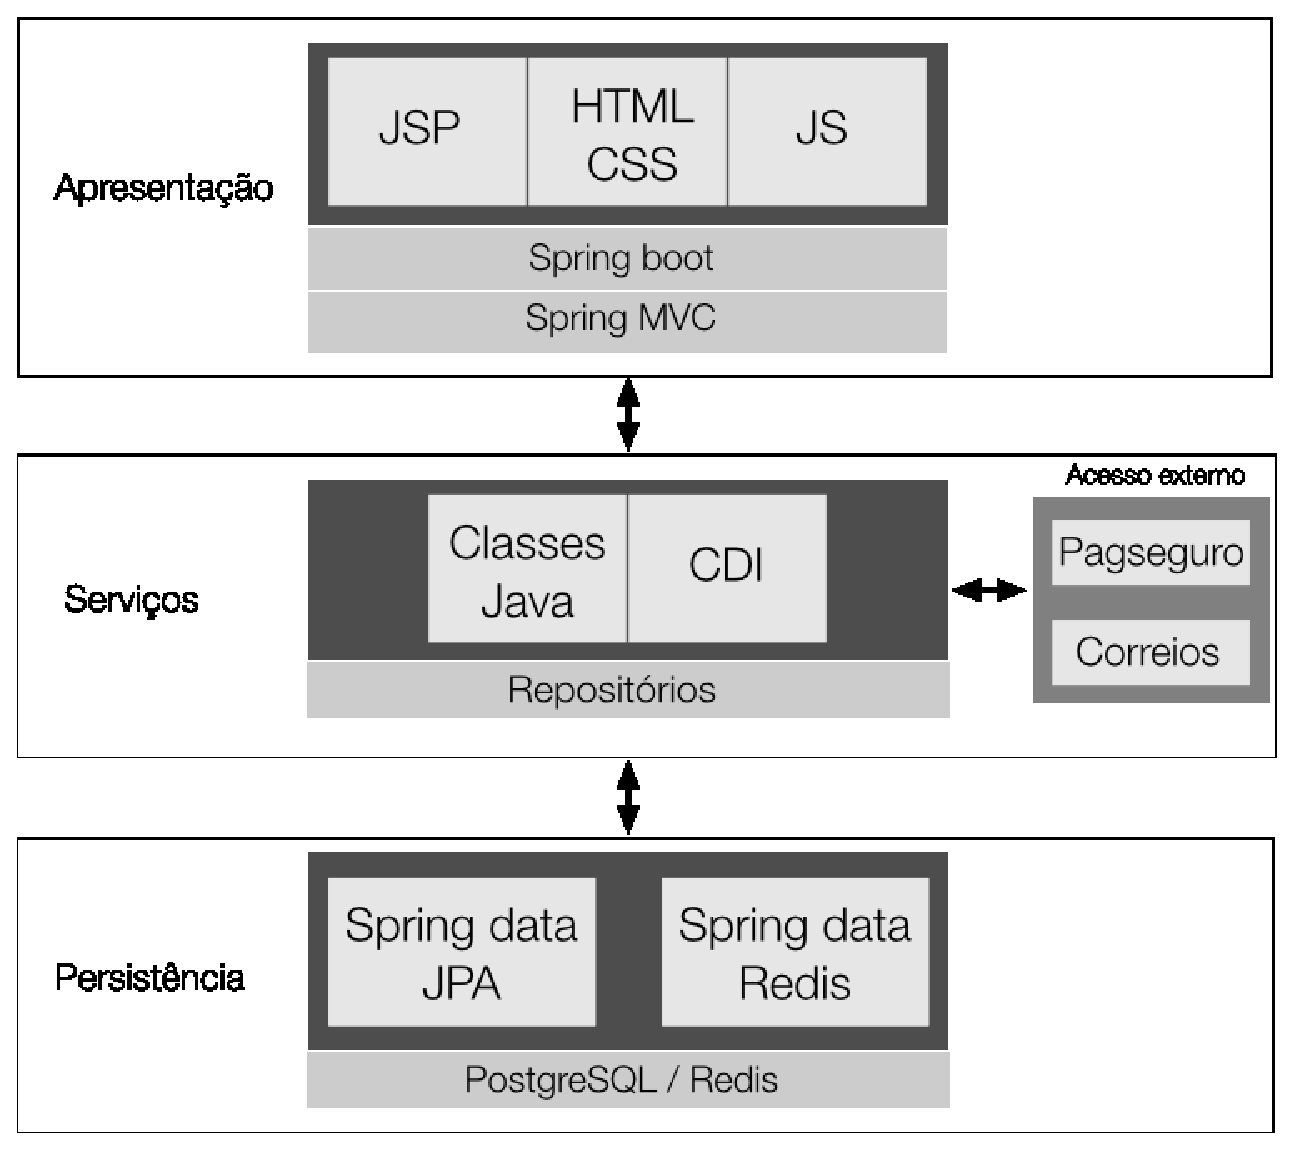
\includegraphics[scale=0.5]{img/representacao-pa.eps}
% \caption{Modelo em camadas do Sudo Loja}
% \label{fig:representacao-pa}
% \end{figure}

% \subsection{Camada de Apresentação} % (fold)
% \label{sub:camada_de_apresentacao}

% A partir desta camada o usuário poderá interagir diretamente com o sistema. Será composta por páginas JSP (\textit{Java Sever Pages}) e HTML(\textit{HyperText Markup Language}, que significa Linguagem de Marcação de Hipertexto), estas que serão estilizadas com o uso de CSS3. Para agilizar o processo de desenvolvimento dessas páginas, será usado o \textit{framework} \textit{Bootstrap} na versão 3. Com isso, a velocidade na criação das páginas aumentará devido a existência de dezenas de componentes já estilizados e estruturalmente organizados, que poderão ser reaproveitados. Alguns efeitos visuais da página serão implementados com o uso de \textit{JavaScript}. Todo conteúdo dinâmico dessas páginas serão implementados usando JSP em sua versão 2.1 e para o conteúdo estático será usado HTML.

% Dois módulos serão implementados para esta camada. O módulo de gerenciamento do sistema, utilizado pelo Lojista e o módulo Loja Virtual que será utilizado pelos Clientes. O módulo gerenciamento irá conter as páginas de gerenciamento da Loja Virtual. E o módulo Loja Virtual as páginas para acesso dos clientes.

% Esta camada poderá interagir diretamente (e apenas) com sua camada adjacente, a camada de Serviços que será discutida na seção \ref{sub:camada_de_servicos}.O estabelecimento desta comunicação será feita utilizando a API (\textit{Application Programming Interface}, no português Interface de Programação de Aplicação ) de \textit{Servlets} em sua versão 3.0, todas as páginas irão fazer requisições a um único \textit{servlet}, este irá chamar o serviço apropriado dependendo do comando recebido na requisição.

% % subsection camada_de_apresentacao (end)

% \subsection{Camada de Serviços} % (fold)
% \label{sub:camada_de_servicos}

% Esta camada fornecerá todos os serviços necessários para o funcionamento do sistema. Terá acesso direto às suas camadas adjacentes: Camada de Apresentação e Camada de Persistência. Para isso, fará uso da linguagem de programação Java. É composta por um conjunto de classes Java, cada qual com suas responsabilidades. Estas classes validarão e manipularão os dados vindo da camada de apresentação. Essas classes que fornecerão os serviços, irão acessar diretamente a camada de persistência, esta que por sua vez irá retornar algum resultado, para que o serviço realize o processamento e retorne para a camada de apresentação.

% Dois módulos serão implementados para esta camada. O módulo de serviços inerentes as operações do modulo de gerenciamento, este que poderá conter outros módulos como um módulo de personalização que fornecerá serviços para gerenciamento do layout; E um modulo de serviços inerentes as operações do modulo Loja Virtual. Um módulo de vendas responsável por prover os serviços inerentes a venda também fará parte do módulo Loja Virtual.

% % subsection camada_de_servicos (end)

% \subsection{Camada de Persistência} % (fold)
% \label{sub:camada_de_persistencia}

% Esta camada será responsável por manter e disponibilizar todos os dados do sistema. Para isto terá auxílio do provedor \textit{EclipseLink}, implementação da especificação JPA 2.0. Estas ferramentas automatizarão o processo criação das tabelas relacionais do banco de dados (onde será usado o \textit{PostgreSQL}), e auxiliarão  nas operações CRUD (acrônimo de \textit{Create}, \textit{Read}, \textit{Update} e \textit{Delete} na língua Inglesa) para as quatro operações básicas utilizadas em bases de dados relacionais (RDBMS) criação, consulta, atualização e exclusão de dados.

% % subsection camada_de_persistencia (end)

% \subsection{Diagrama de Componentes} % (fold)
% \label{sub:diagrama_de_componentes}

% Para possibilitar uma melhor compreensão da arquitetura do sistema, a Figura \ref{fig:cd} apresentará através de um diagrama de componentes, os módulos que irão existir em cada camada.

% \begin{figure}[H]
% \centering
% 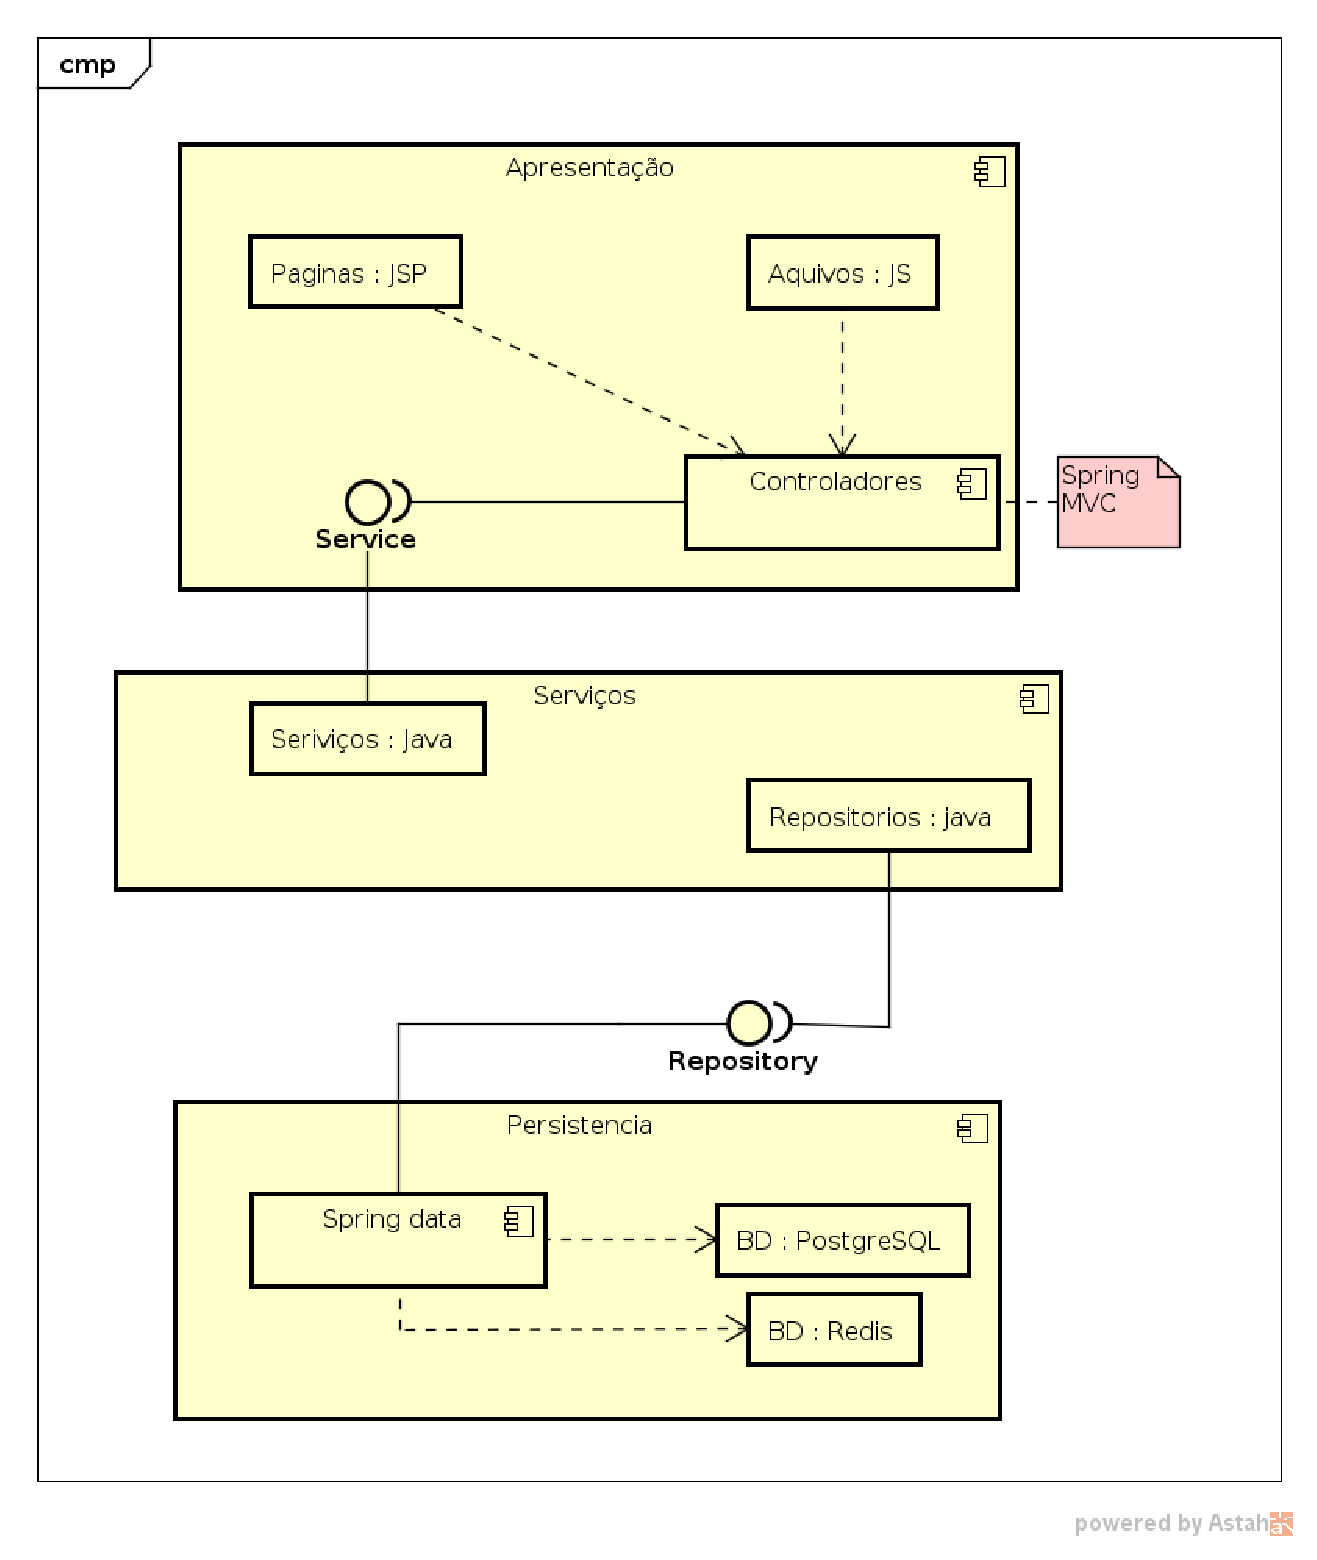
\includegraphics[width=14cm]{img/diagramas/cd.eps}
% \caption{Diagrama de Componentes do Sistema}
% \label{fig:cd}
% \end{figure}


% % subsection diagrama_de_componentes (end)

% \subsection{Tecnologias Utilizadas} % (fold)
% \label{sub:tecnologias_ultilizadas}

% Está seção apresentará com detalhes todas as tecnologias que serão utilizadas no sistema.

% \begin{itemize}
% \item \textbf{HTML} - No HTML (Hypertext Markup Language) ou Linguagem de Marcação de Hipertexto são definidos símbolos de marcação que informam ao navegador World Wide Web como exibir textos, imagens e uma variedade de recursos na página que é renderizada e apresentada ao usuário \cite{html}.

% \item \textbf{JSP e Servlets} - \textit{JavaServer Pages} (JSP) e Servlets são tecnologias complementares para a produção páginas Web dinâmicas via Java. Servlets são a base para o \textit{server side} Java. JSP complementa Servlets  simplificando o desenvolvimento. Uma página JSP básica consiste em texto simples e de marcação e pode, opcionalmente, ter scripts incorporados e outras funcionalidades para a criação dinâmica de conteúdo \cite{jsp2007java}.

% \item \textbf{CSS} - Cascading Style Sheets (CSS) é uma “folha de estilo” composta por “camadas” e utilizada para definir a apresentação (aparência) em páginas da internet que adotam para o seu desenvolvimento linguagens de marcação (como XML, HTML e XHTML). O CSS define como serão exibidos os elementos contidos no código de uma página da internet e sua maior vantagem é efetuar a separação entre o formato e o conteúdo de um documento \cite{anapereira}.

% \item \textbf{JavaScript} - A linguagem Javascript é executada no navegador e trabalha juntamente com o mesmo de forma a tornar as páginas estáticas em páginas dinâmicas \cite{goodman}. É uma linguagem popular e hoje é empregada em diversas plataformas,tal como cliente, servidor, smartphones e desktops \cite{stefanov}.

% \item \textbf{Bootstrap} - Originalmente criado por um designer e um desenvolvedor do Twitter \citeyear{twitter}, o \textit{Bootstrap} é um framework front-end popular e é um projeto de código aberto. O \textit{Bootstrap} em sua terceira versão se preocupa primeiramente com acesso por dispositivos móveis, focando-se no design responsivo \cite{bootstrap}.

% \item \textbf{Java} - Originalmente desenvolvida por uma equipe de desenvolvedores liderada por James Gosling na \textit{Sun Microsystems} (atualmente de propriedade da Oracle) e lançada em 1995, o Java é uma linguagem de programação orientada a objetos que atualmente faz parte do núcleo da Plataforma Java \cite{java}.

% \item \textbf{JPA} - JPA é um framework leve, baseado em POJOS (Plain Old Java Objects) para persistir objetos Java. A Java Persistence API, diferente do que muitos imaginam, não é apenas um framework para Mapeamento Objeto-Relacional (ORM - Object-Relational Mapping), ela também oferece diversas funcionalidades essenciais em qualquer aplicação corporativa \cite{medeiros}.

% \item \textbf{PostgreSQL} - PostgreSQL é um sistema poderoso banco de dados objeto-relacional open source. Ele tem mais de 15 anos de desenvolvimento ativo e uma arquitetura comprovada que ela ganhou uma forte reputação de confiabilidade, integridade de dados e correção. Ele é executado em todos os principais sistemas operacionais, incluindo Linux, UNIX (AIX, BSD, HP-UX, SGI IRIX, Mac OS X, Solaris, Tru64), e Windows. É totalmente compatível com ACID, tem suporte completo para chaves estrangeiras, junções views, triggers e procedimentos armazenados (em várias línguas). Ele inclui mais 2008 tipos de dados SQL, incluindo INTEGER, NUMERIC, BOOLEAN, CHAR, VARCHAR, DATE, INTERVAL e TIMESTAMP. Ele também suporta o armazenamento de grandes objetos binários, incluindo imagens, sons ou vídeo. Ele tem interfaces de programação nativas para C / C ++, Java, .Net, Perl, Python, Ruby, Tcl, ODBC, entre outros, e documentação excepcional \cite{postgresql}.

% \end{itemize}

% % subsection tecnologias_ultilizadas (end)

% \subsection{O Que Deve Ser Produzido} % (fold)
% \label{sub:o_que_deve_ser_produzido}

% Como o sistema será web e utilizará Java como linguagem \textit{server side} o sistema deverá funcionar em um servidor para sistemas  Java. Para o desenvolvimento será  utilizado o \textit{containner} Apache Tomcat 7.0. 

% Quanto ao processo de instalação, basta que o arquivo .war gerado no \textit{deploy} da aplicação seja colocado dentro da pasta do servidor. No caso do Tomcat esta pasta é chamada de “WebApps”. Após implantado nesta pasta, basta iniciar o \textit{containner} e acessar a URL do mesmo / (barra) o nome da aplicação.

% % subsection o_que_deve_ser_produzido (end)

% % section projeto_arquitetural (end)

% \section{Diagrama de Classes} % (fold)
% \label{sec:diagrama_de_classes}

% Na Figura \ref{fig:diagrama-classe-estoque}, será apresentado um diagrama de classes que ilustra uma visão mais baixo nível de como as classes necessárias para realizar as operações da US03, deverão se comunicar. 

% \begin{figure}[H]
% \centering
% 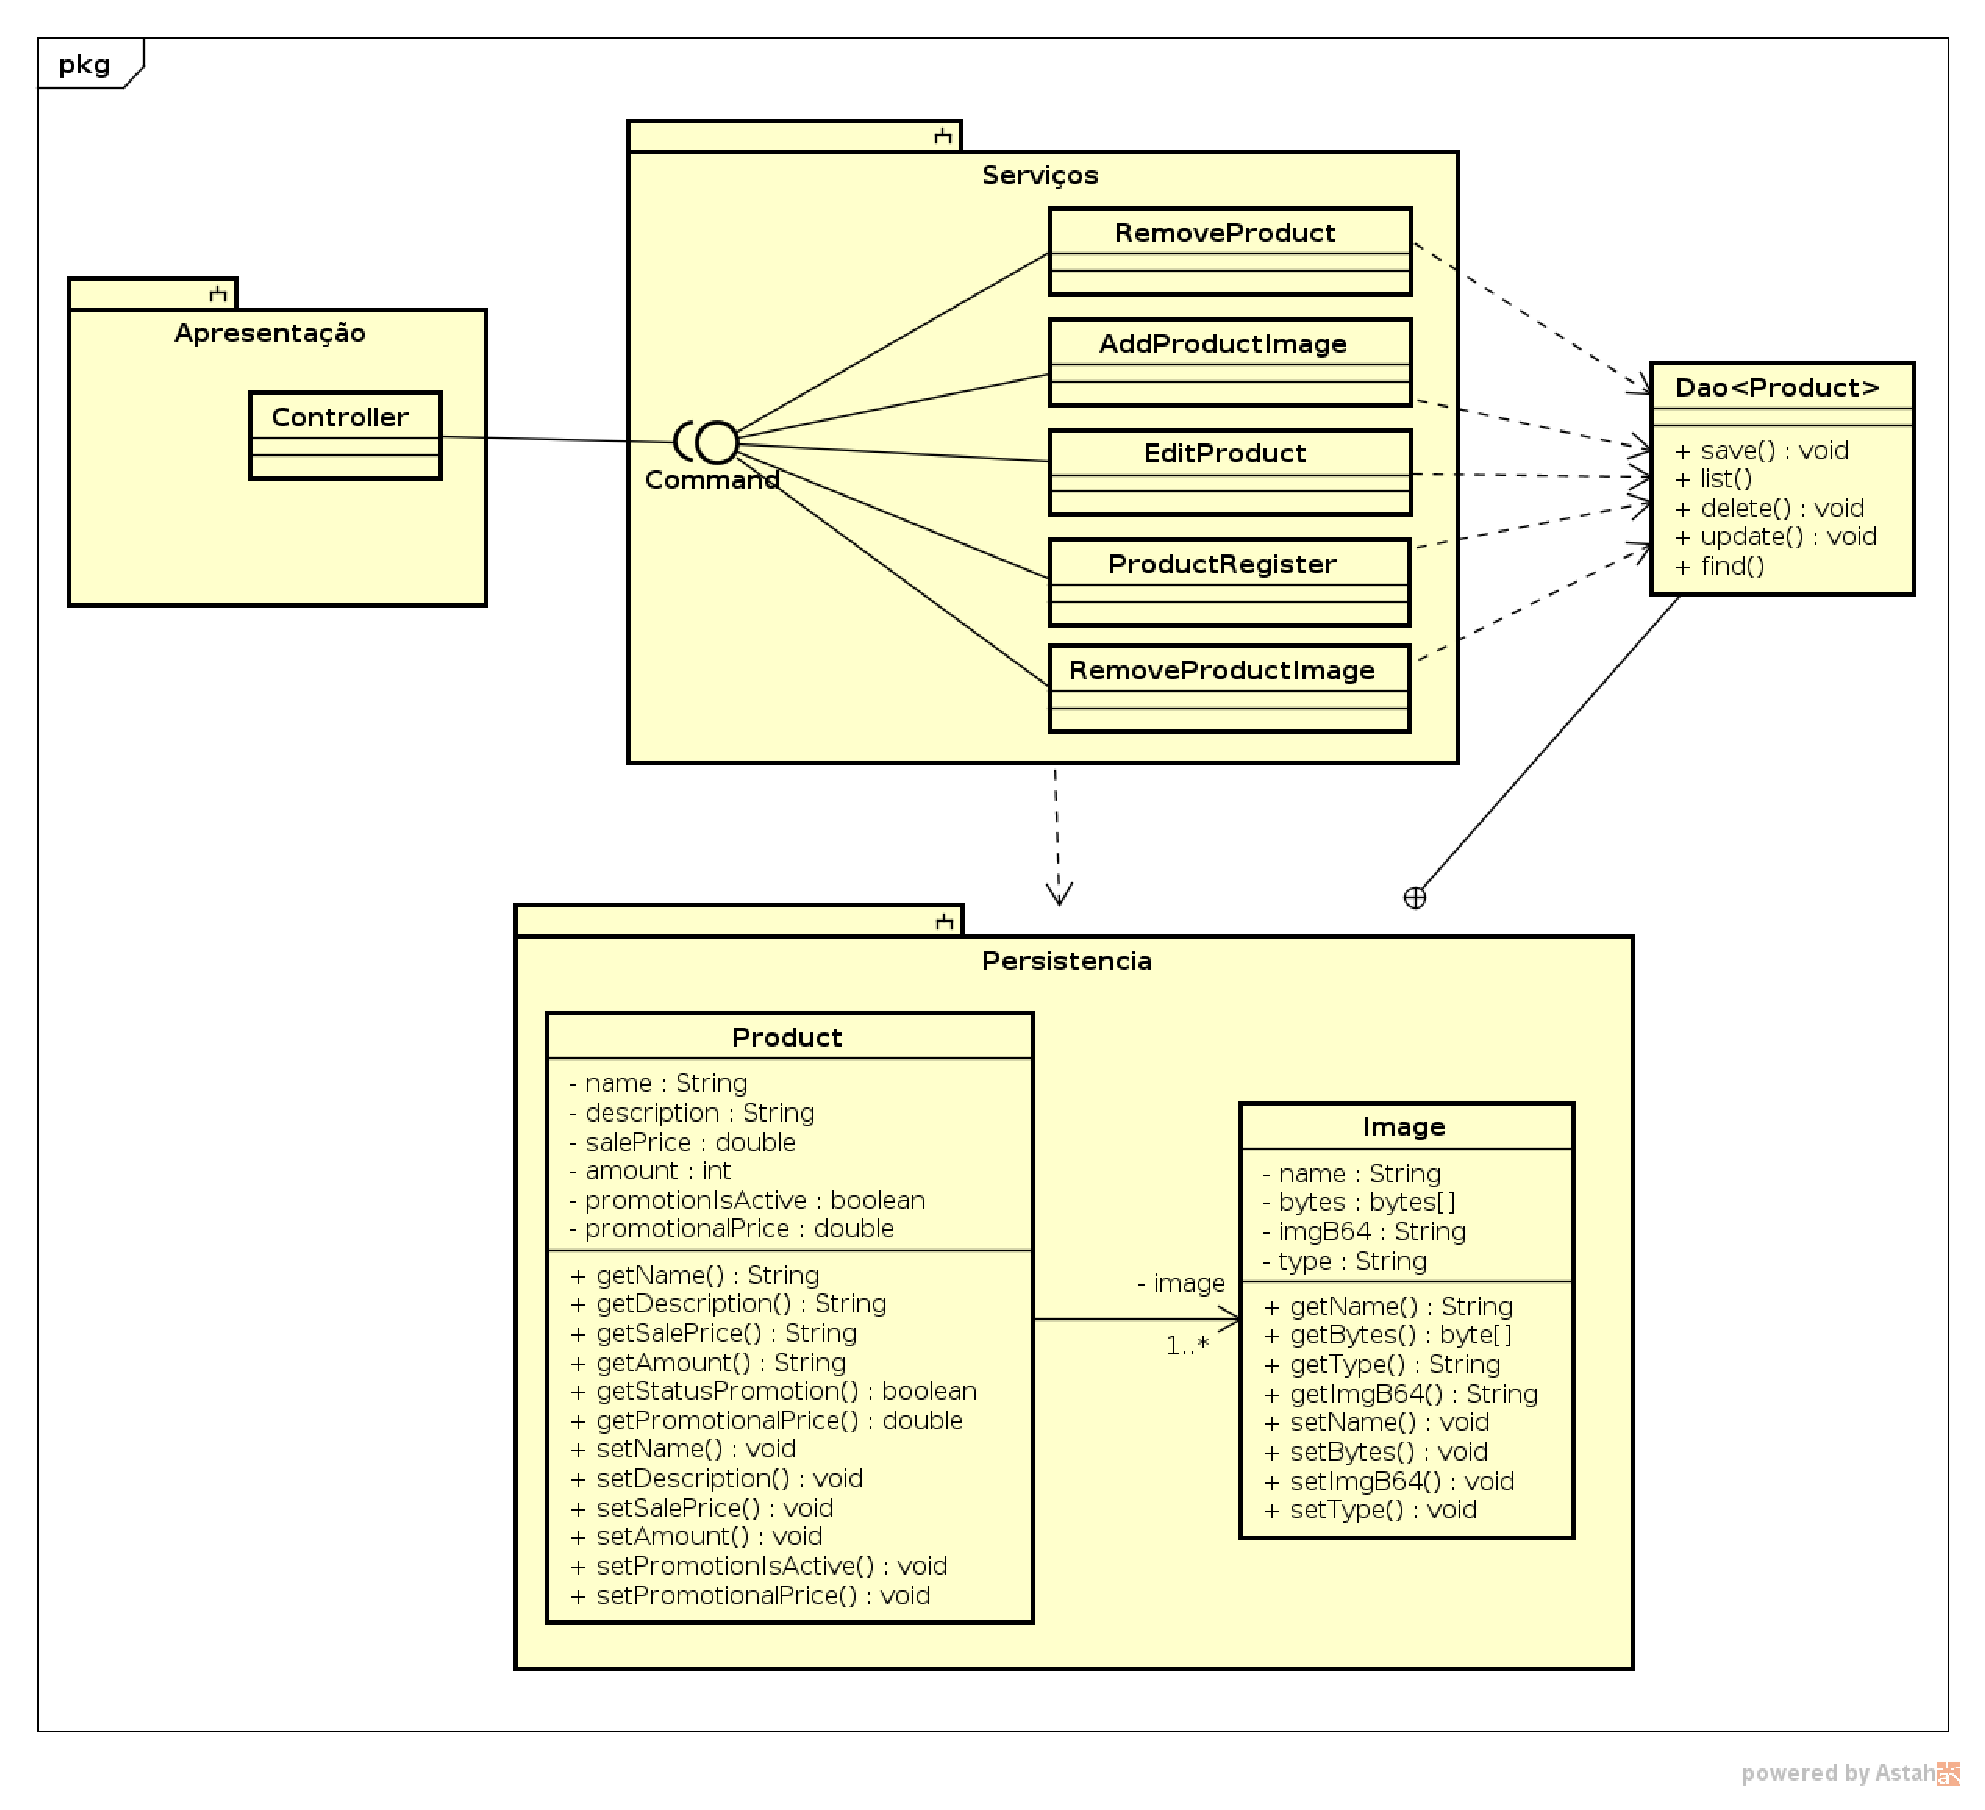
\includegraphics[width=14cm]{img/diagramas/class-diagram-estoque.eps}
% \caption{Diagrama de classes US03}
% \label{fig:diagrama-classe-estoque}
% \end{figure}

% A classe Controller ainda na camada de apresentação invocará um comando apropriado na camada de serviços, que fará uso da Classe Dao na camada de persistência que por sua vez retornará para o serviço o resultado que será repassado para a apresentação.

% % section diagrama_de_classes (end)

% \section{Implementação} % (fold)
% \label{sec:implementacao}

% Na Figura \ref{fig:sd-atualiza}, será apresentado um diagrama de sequência que ilustra como se dá a atualização de um produto do estoque, tarefa esta que faz parte da US03.

% \begin{figure}[H]
% \centering
% 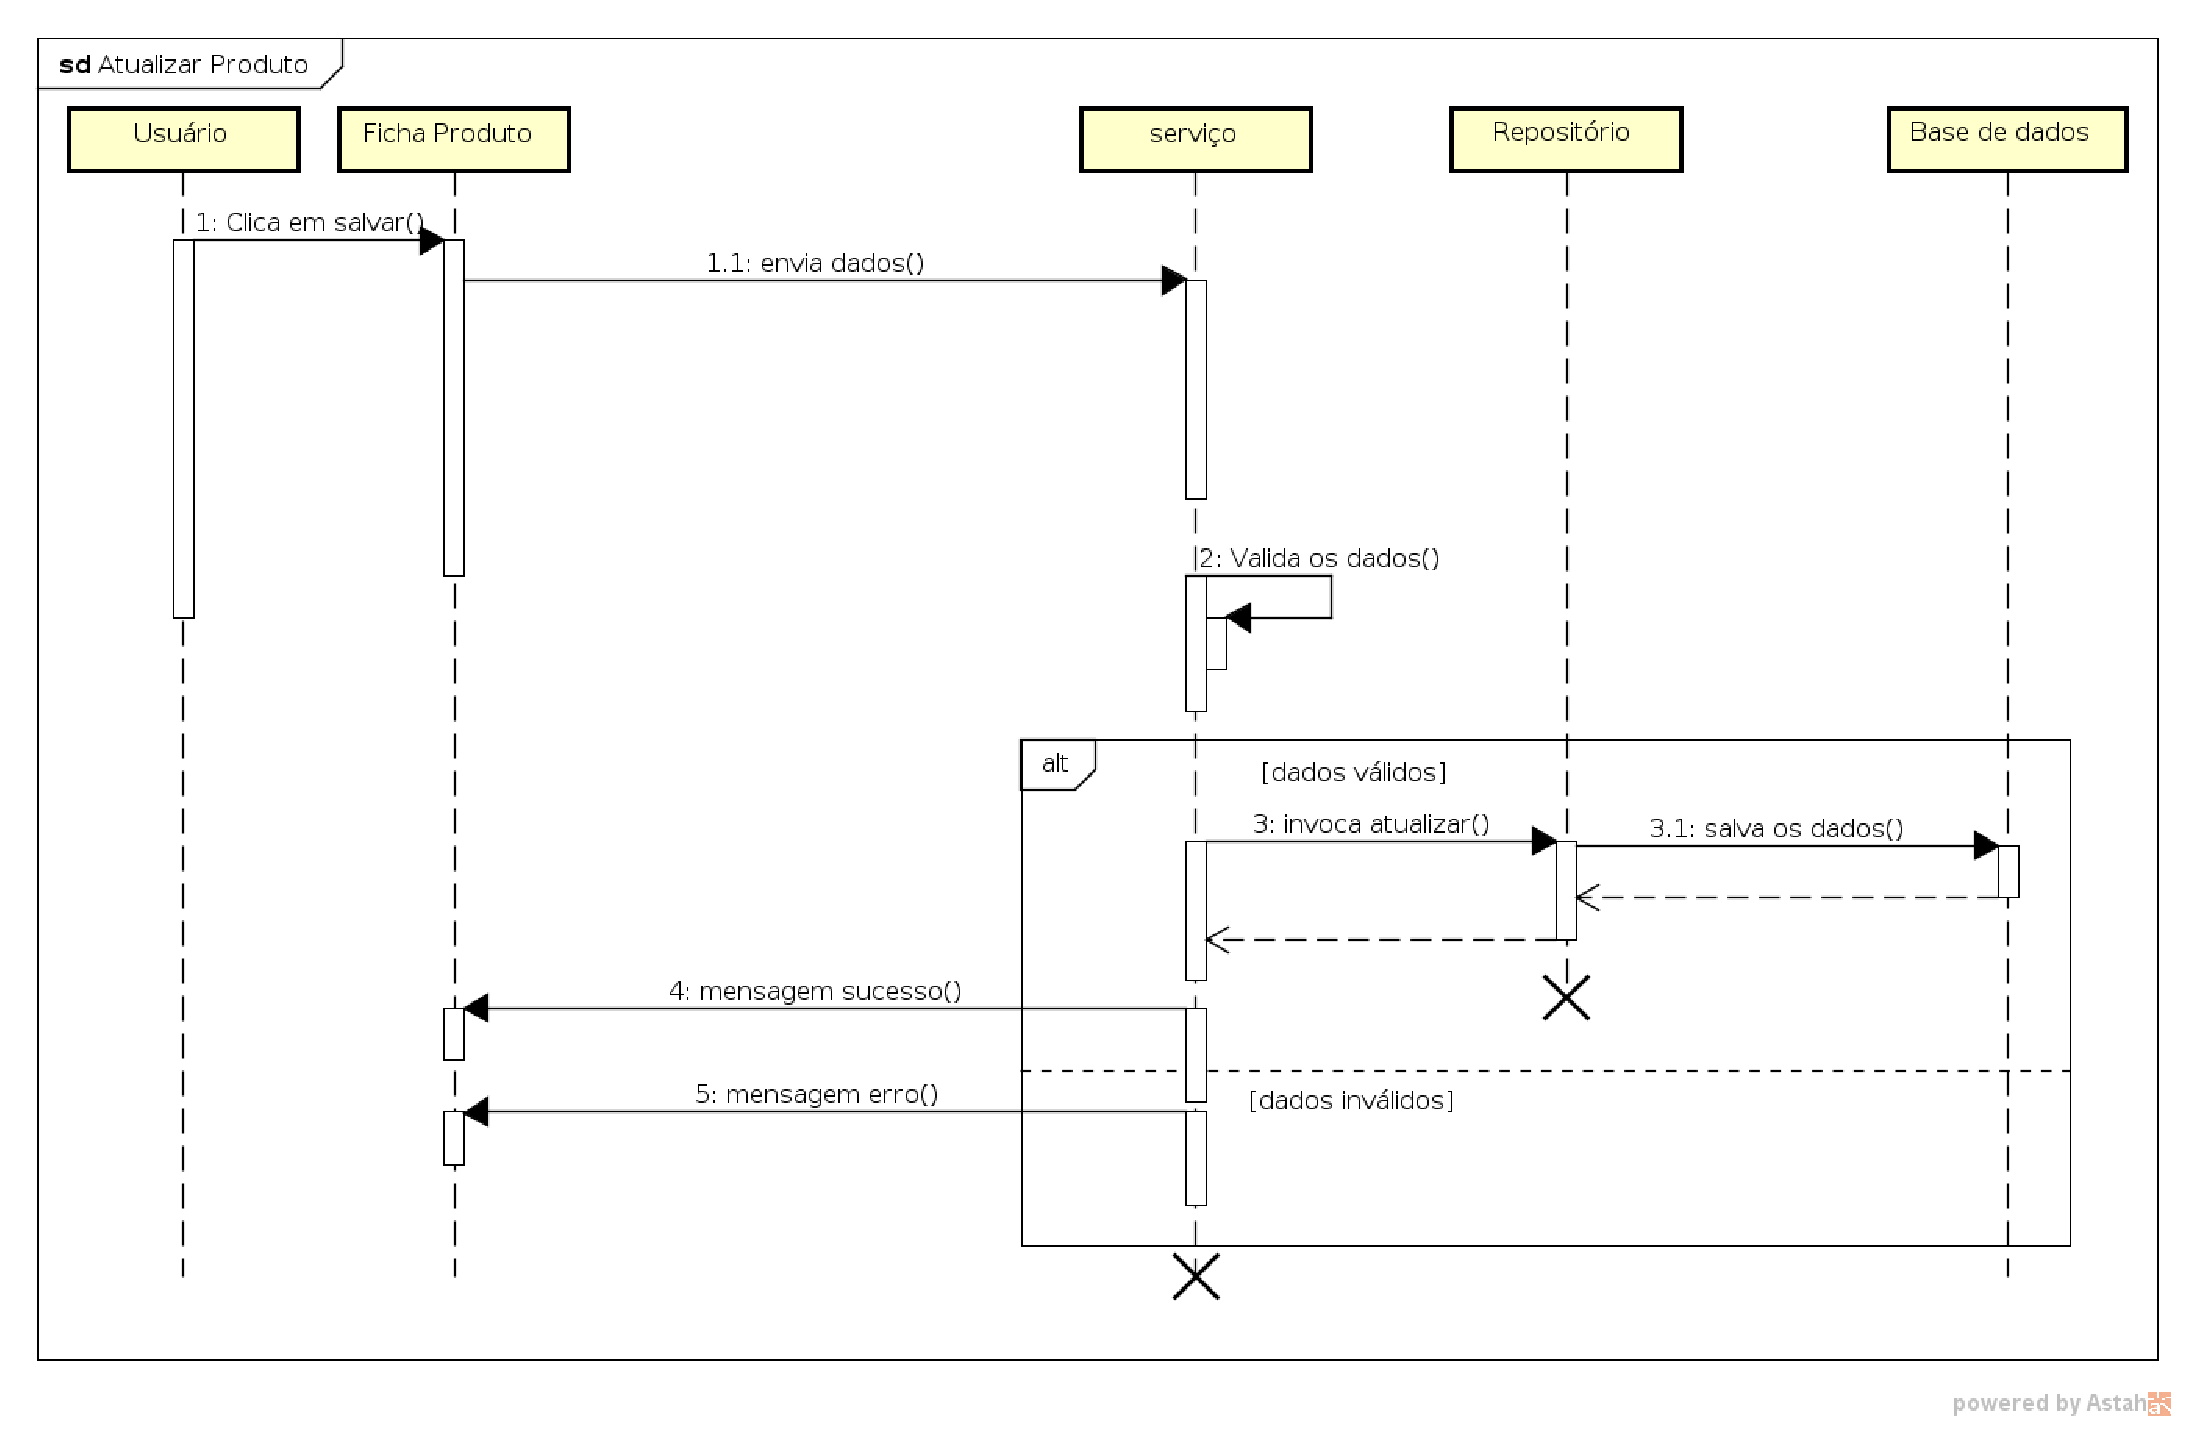
\includegraphics[width=15cm]{img/diagramas/sd-atualiza-produto.eps}
% \caption{Diagrama de sequência - atualizar informações do Produto}
% \label{fig:sd-atualiza}
% \end{figure}

% Suponhamos que o usuário já esteja devidamente cadastrado e logado no sistema e agora está na página de edição de um produto do estoque, como representa a figura \ref{fig:ficha-produto}. O usuário altera as informações que jugar necessário e clica no botão salvar, isto gera uma requisição para o servlet controlador, que por sua vez irá invocar o serviço de atualizar produto. Antes de salvar as alterações o serviço irá validar os dados, sendo válidos o Dao de produto é invocado e as alterações são salvas na base de dados e será exibida uma mensagem de sucesso na tela. Caso as informações não sejam válidas será apresentada uma mensagem de erro na mesma tela.

% \begin{figure}[H]
% \centering
% 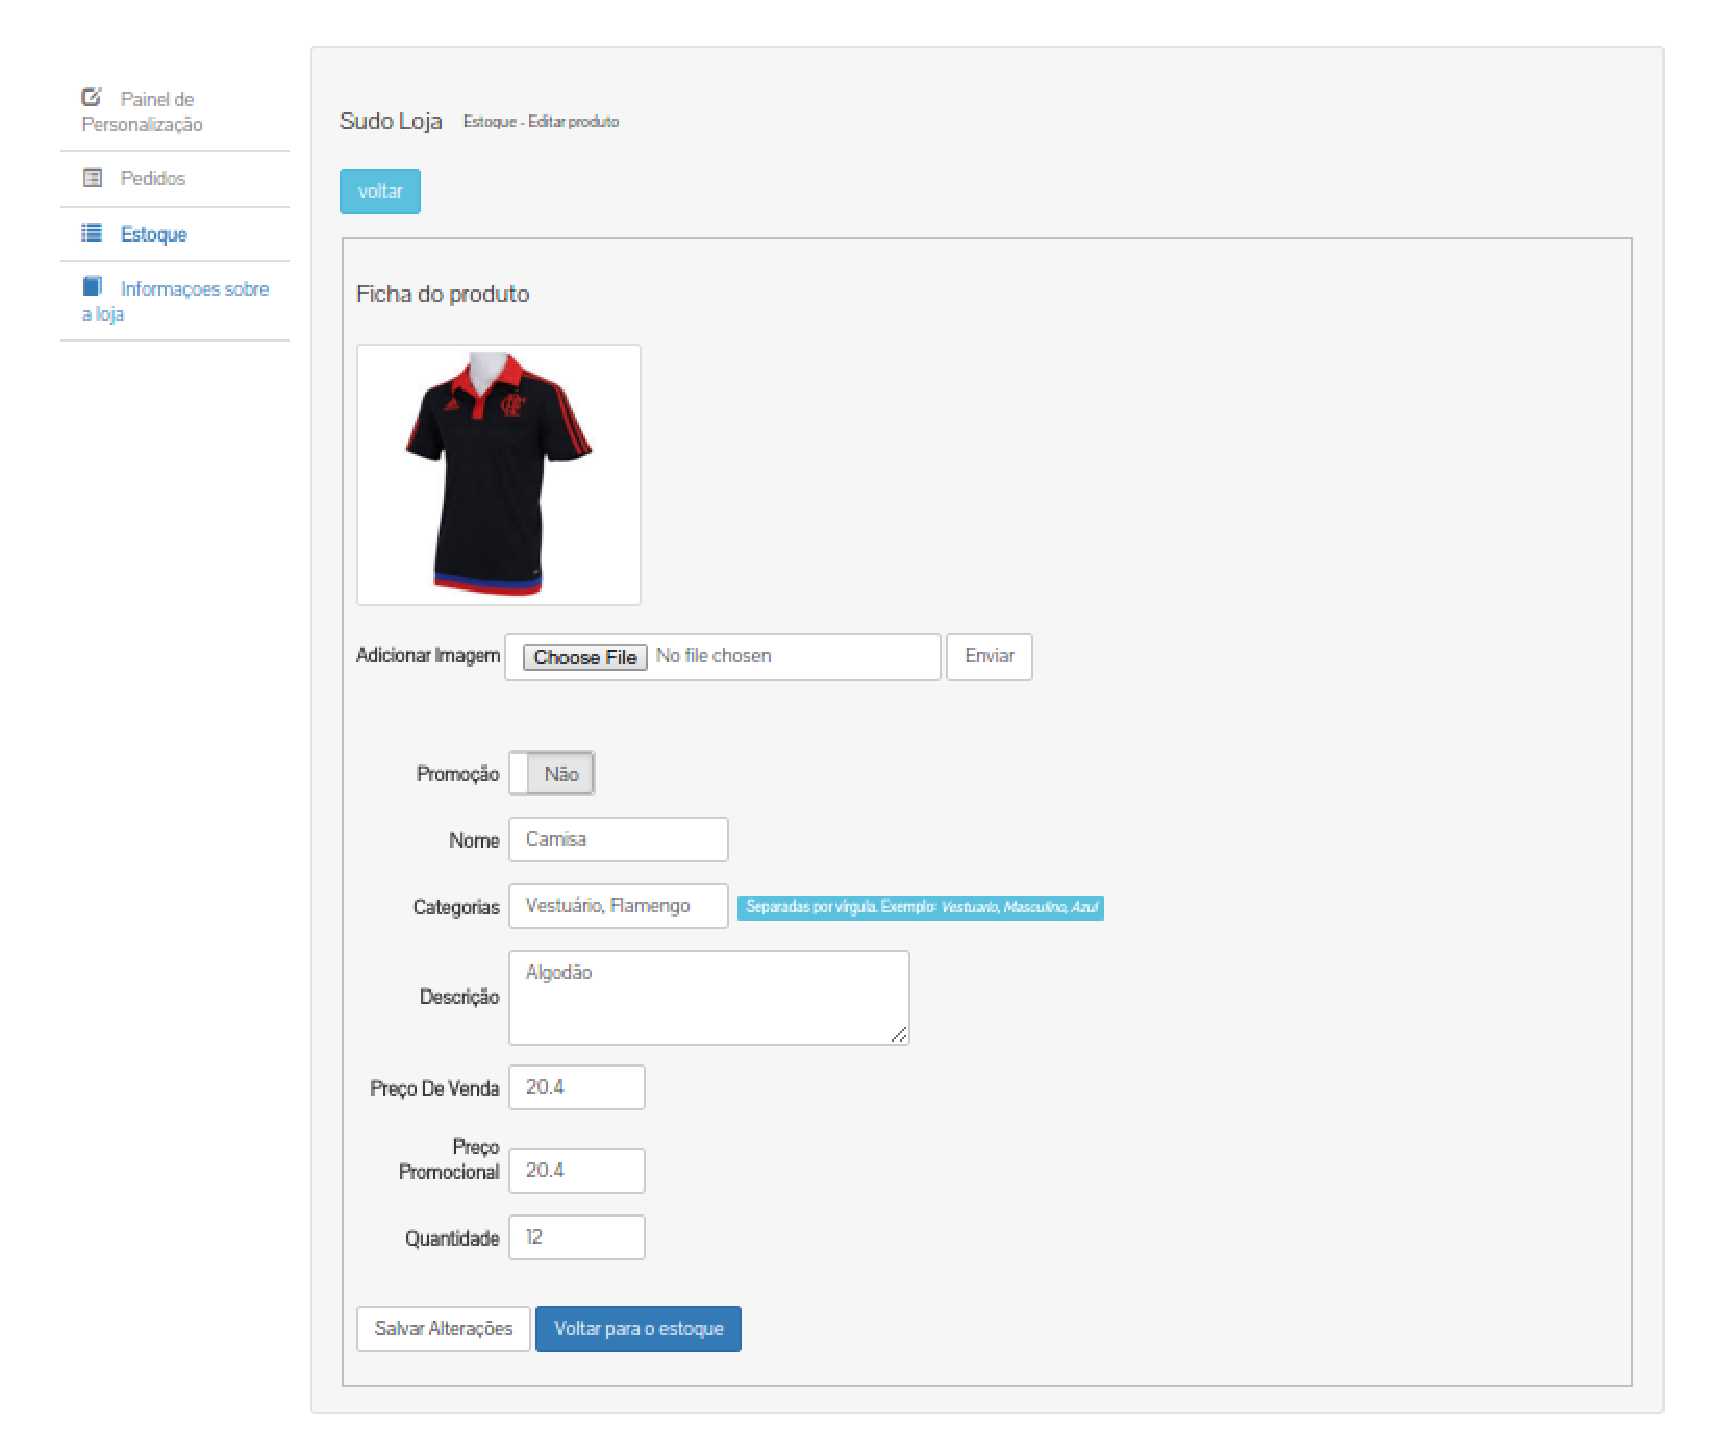
\includegraphics[width=15cm]{img/sistema/ficha-produto.eps}
% \caption{Ficha de edição de Produto}
% \label{fig:ficha-produto}
% \end{figure}

% O estoque de uma loja do sistema é ilustrado na Figura \ref{fig:sistema-estoque}. Nessa página o usuário pode adicionar um novo produto, clicando no botão \textbf{Novo Produto}, onde será exibido um formulário para inserção dos dados do produto; Poderá também editar um produto, clicando sobre o botão destacado em azul com descrição \textbf{Ficha}, exibindo uma ficha, onde o usuário poderá ver com detalhes todas as informações inerentes ao produto, podendo atualizá-las; E excluir um produto clicando sobre o botão destacado na cor vermelha com descrição \textbf{Excluir}, onde será exibida uma janela para confirmar a operação, resultando ou não na exclusão do produto. 

% \begin{figure}[H]
% \centering
% 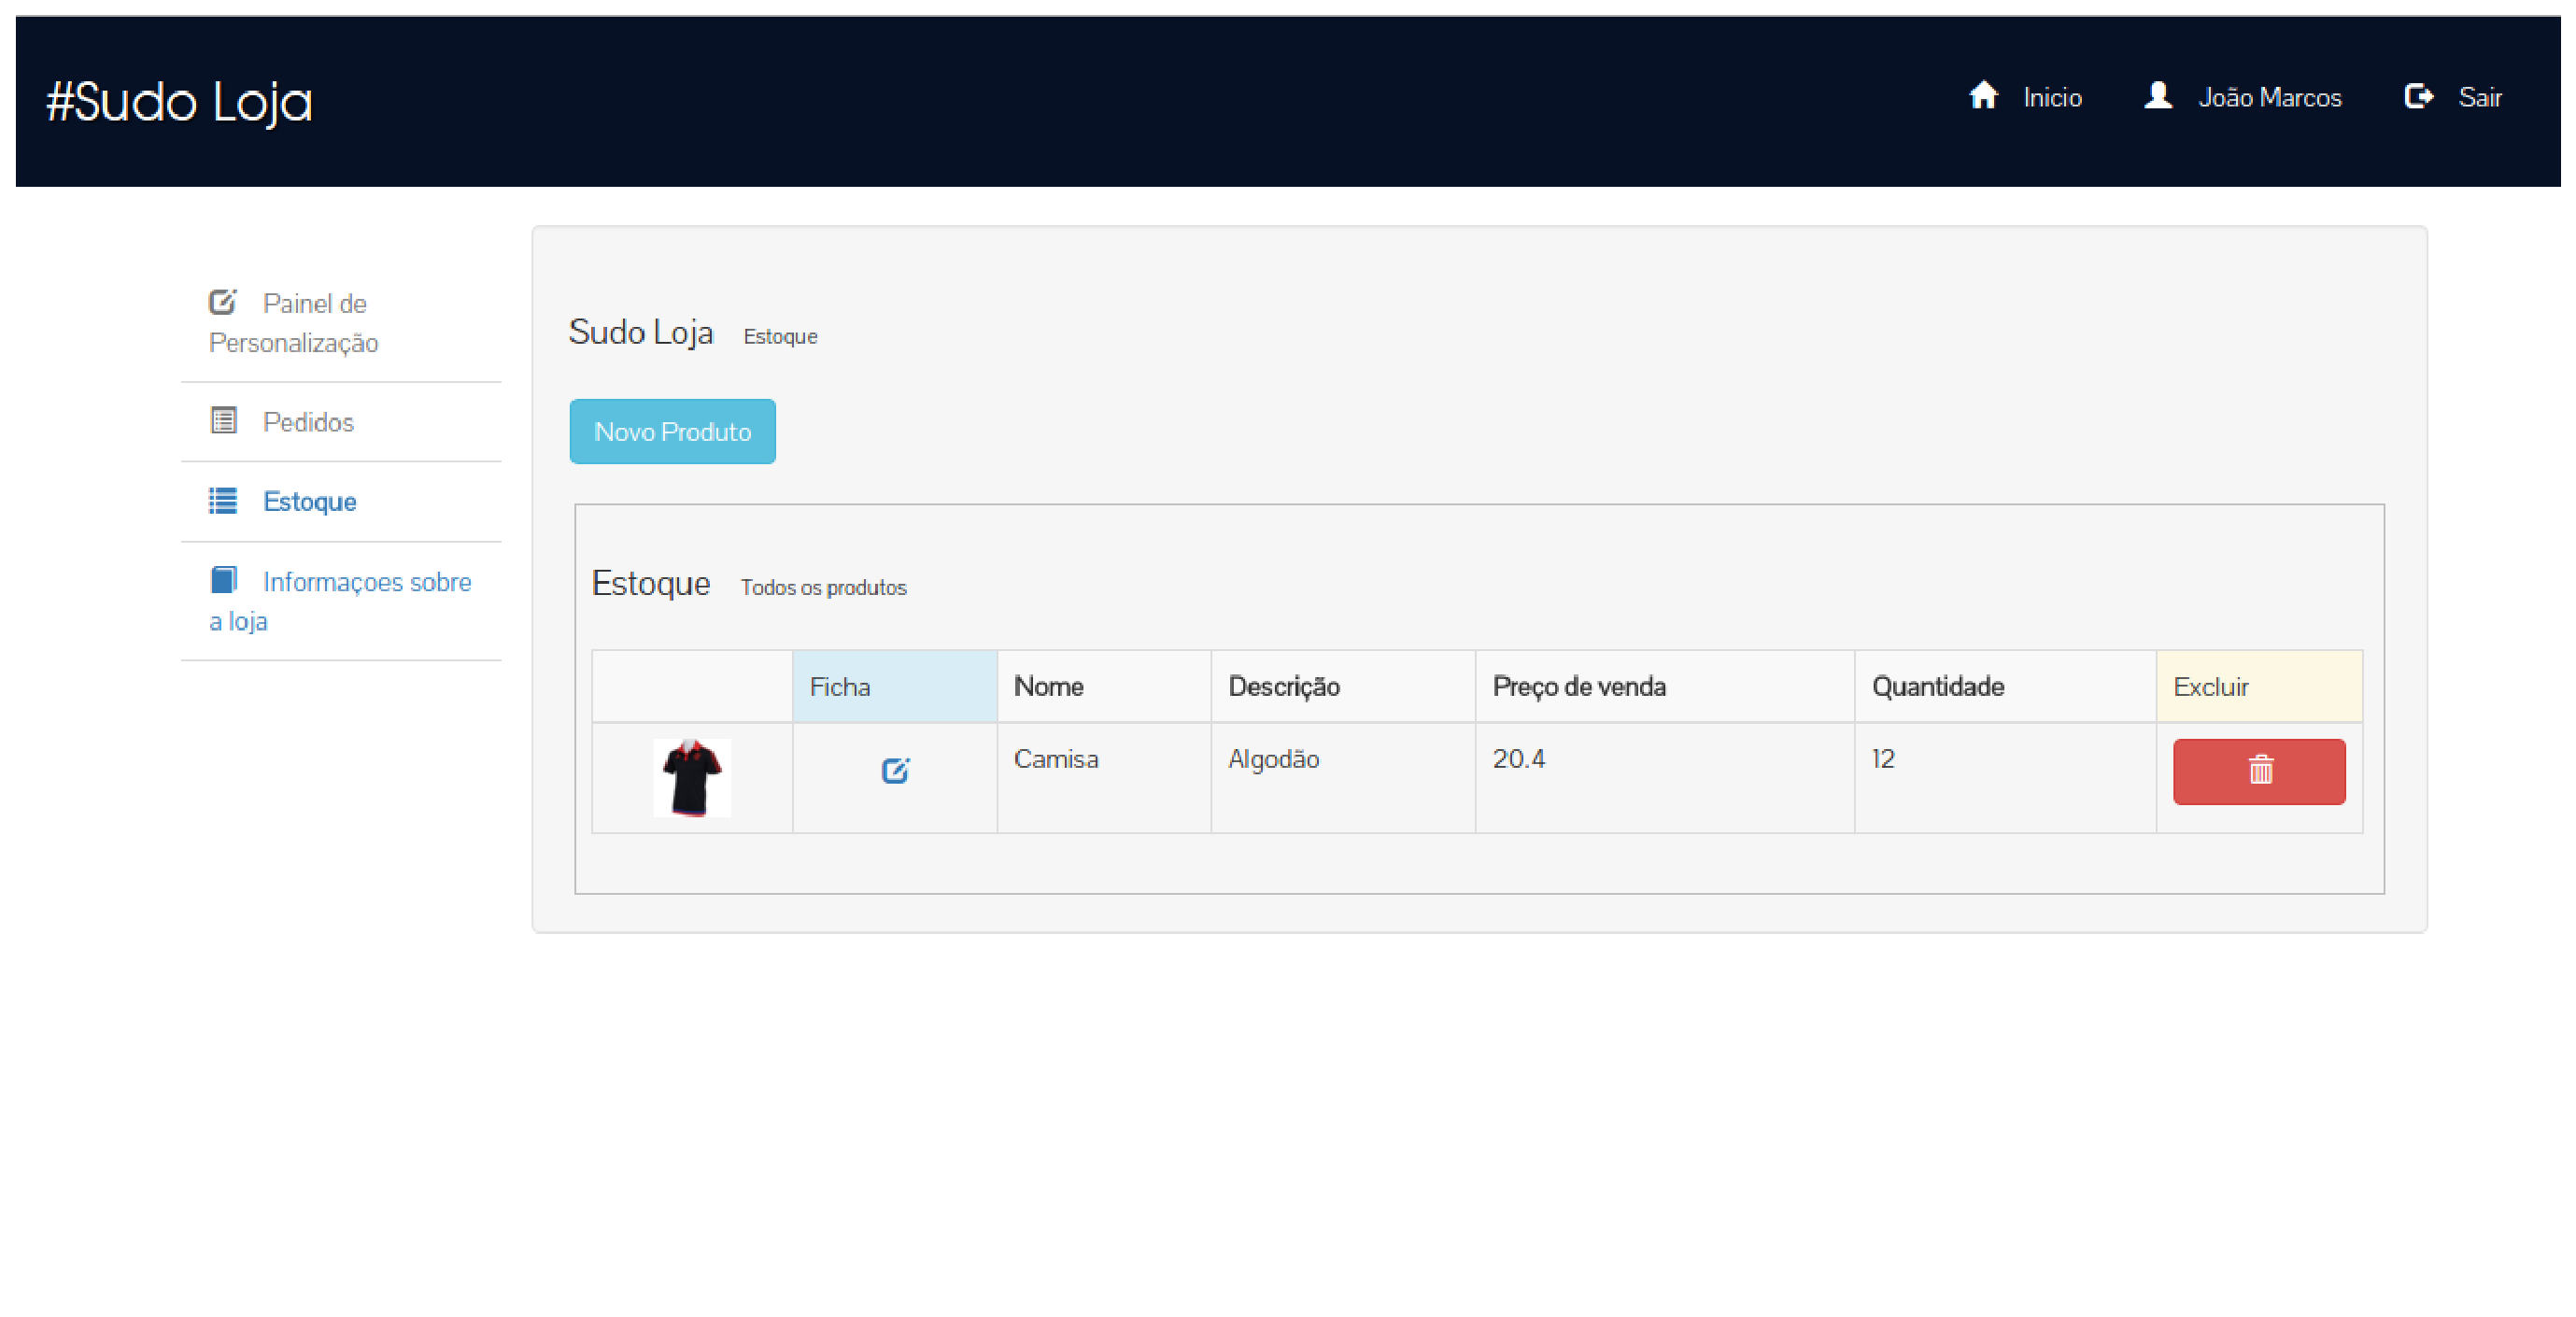
\includegraphics[width=15cm]{img/sistema/pagina-estoque.eps}
% \caption{Página do estoque de uma loja do sistema}
% \label{fig:sistema-estoque}
% \end{figure}


% section implementacao (end)
% chapter o_sistema (end)


% chapter sudo_loja (end)

\bibliography{referencias}

% Inicio do Apêndice
\appendix
\newpage
\phantomsection
\addcontentsline{toc}{chapter}{Apêndices}  
\addtocontents{toc}{\protect\setcounter{tocdepth}{-1}}
\chapter{Documento de Visão}
\label{ap:documento_visao}
\section{Introdução} % (fold)
\label{sec:Introducao}

Este documento apresenta uma solução de software para ser apresentado como TCC, solicitado pelos professores. Como cliente Francisco Paulo de Freitas Neto (Orientador). Apresenta também os problemas a serem solucionados, as necessidades dos principais envolvidos, o alcance do projeto e as funcionalidades esperadas do sistema.

\subsection{Objetivos} % (fold)
\label{sec:objetivos}

Como objetivo principal, esse projeto visa facilitar o ingresso de um comerciante ao mercado virtual, fornecendo uma ferramenta capaz de criar uma loja virtual onde um usuário, sem ajuda especializada, poderá gerenciar e customizar sua loja de maneira simples e intuitiva.

% subsection objetivos (end)

\subsection{Abrangência do Projeto} % (fold)
\label{sec:abrengencia_do_projeto}

Esse projeto é voltado ao âmbito comercial, contemplando todos aqueles que desejam criar uma loja virtal e disponibilizar produtos à venda.
O produto final será uma plataforma onde qualquer usuário cadastrado poderá criar, gerenciar e personalizar uma loja virtual.

% subsection abrengencia_do_projeto (end)

\subsection{Definições, Acrônimos e Abreviações} % (fold)
\label{sec:siglas}

\textbf{CMS} – Content Management System (Sistema de Gerenciamento de Conteúdo)

% subsection siglas (end)
\subsection{Organização do Documento} % (fold)
\label{sec:organizacao_do_documento}

As próximas seções trataram sobre a descrição do problema, as partes envolvidas e tipos de usuários que utilizaram o sistema, a solução proposta para os problemas elencados, logo após, as funcionalidades oferecidas por esta solução, seguidas pelas restrições do sistema. Também poderão ser vistos alguns protótipos na Seção \ref{sec:prototipos}.

% subsection organizacao_do_documento (end)
% section Introdução (end)

\section{Descrição do Problema} % (fold)
\label{cha:descricao_do_problema}

\begin{itemize}
\item Dificuldades no gerenciamento de uma loja virtual - 
Aqueles que desejam entrar no mercado virtual geralmente recorrem a empresas de desenvolvimento de software para criar sua loja virtual, e geralmente, qualquer tipo de modificação a ser feita, seja no conteúdo ou no \textit{layout} e estilo do site, necessita da intervenção direta da equipe de desenvolvimento.

\item Afeta - O lojista.
\item O impacto deste problema é - 
Um grande impacto que isso causa para o lojista é a demora, tanto no desenvolvimento quanto na modificação de alguma parte da loja online, por exemplo, digamos que por algum motivo o lojista queira modificar o estilo do sua loja online. A equipe então, levará um certo tempo (dependendo da complexidade de modificação) até entender completamente o que o cliente deseja para então realizar a modificação e deixar a loja do jeito que o cliente pediu, e é claro, na maioria dos casos com um custo considerável. Então temos dois problemas principais: demora e custo.

\item Uma solução ideal permitiria - 
Fornecer um sistema que possibilitasse a criação, personalização  e gerenciamento de uma loja online sem intervenção de pessoal especializado, com um baixo custo.

\end{itemize}

% section descricao_do_problema (end)

\section{Partes Envolvidas} % (fold)
\label{sec:partes_envolvidas}

Os principais envolvidos serão descritos nas seções \ref{sec:resumo_dos_envolvidos} e \ref{sec:resumo_dos_usuarios}.

\subsection{Resumo dos Envolvidos} % (fold)
\label{sec:resumo_dos_envolvidos}

Os envolvidos que se interessam em empenhar-se nesse projeto, são os desenvolvedores, os comerciantes, e os consumidores.

% subsection resumo_dos_envolvidos (end)

\subsection{Resumo dos Usuários} % (fold)
\label{sec:resumo_dos_usuarios}

Uma lista resumida de todos os usuários identificados pode ser vista no Quadro \ref{quadro:usuarios}.

\begin{table}[H]
\centering
\caption{Resumo dos usuários}
\label{quadro:usuarios}
\begin{tabular*}{\textwidth}{@{\extracolsep{\fill}} |p{3cm}|p{4cm}|p{4cm}|p{3cm}|}
\hline
\rowcolor{ballblue}
Nome & 	Descrição & Responsabilidades & Envolvido \\
Lojista & Administrador da loja virtual &  Criação da loja, Personalização da loja, Inclusão de dados no sistema, Gerenciamento de pedidos 
& Dono do negócio ou alguém que represente seus interesses \\
\hline
Cliente & Consumidor dos produtos oferecidos na loja & Efetuar cadastro para realização de uma compra & Qualquer consumidor em potencial que deseje  realizar uma compra  (de um ou mais)  produtos oferecidos pela loja \\	
\hline
\end{tabular}
\end{table}

% subsection resumo_dos_usuarios (end)

% section partes_envolvidas (end)

\section{Descrição da Solução Proposta} % (fold)
\label{sec:descri_o_da_solu_o_proposta}

A solução proposta é um sistema computacional web para criação de lojas virtuais (um CMS voltado para criação de lojas, onde um usuário poderá criar, personalizar as suas lojas virtuais e assim, disponibilizar os seus produtos para venda) e uma área para perguntas ao vendedor sobre um produto desejado. tudo isso de forma simples sem conhecimento especializado, sem burocracias. 

% section descri_o_da_solu_o_proposta (end)

\section{Funcionalidades} % (fold)
\label{sec:funcionalidades}

No Quadro \ref{quadro:funcionalidades} podemos ver uma breve descrição das funcionalidades do produto, com um nível de detalhamento genérico para uma melhor compreensão.


\begin{longtable}{|p{7cm}|p{7cm}|}
\caption{Resumo das Funcionalidades}
\label{quadro:funcionalidades}
\hline
\rowcolor{ballblue}
Funcionalidade & Descrição	\\	
Gerenciamento de produtos & Inclusão, remoção e alteração de produtos, cadastro de múltiplas imagens para cada produto
\\	
\hline
Gerenciamento de pedidos & Controle de todos os pedidos realizados
\\	
\hline
Personalização da loja & A loja poderá ser personalizada totalmente (\textit{layout}, cores, fontes, edição de CSS e HTML)
\\	
\hline
Gerenciamento de clientes & Cadastro, alteração de dados cadastrais, remoção da conta.
\\	
\hline
Calculo de frete automático quando houver & Caso haja frete sobre um produto da loja, em tempo real o cliente poderá ver o valor do frete
\\	
\hline
Controle de estoque & O estoque poderá ser consultado e gerenciado, contendo opções como desabilitar/habilitar produtos, visualizar quantidade de cada produto, filtrar produtos por nome
\\	
\hline
Acompanhamento de pedidos para os clientes & Os clientes poderão visualizar o status do pedido a qualquer momento,
\\	
\hline
\end{longtable}	


% section funcionalidades (end)

\section{Restrições do Projeto} % (fold)
\label{sec:restricoes_do_projeto}

O sistema será uma aplicação WEB com design totalmente responsivo, o que significa que poderá ser utilizado tanto pelo navegador de um computador desktop, quanto pelo navegador do celular. Não possuirá restrições quanto ao sistema operacional utilizado pelo consumidor.

% section restricoes_do_projeto (end)

\section{Protótipos} % (fold)
\label{sec:prototipos}

\begin{figure}[H]
\centering
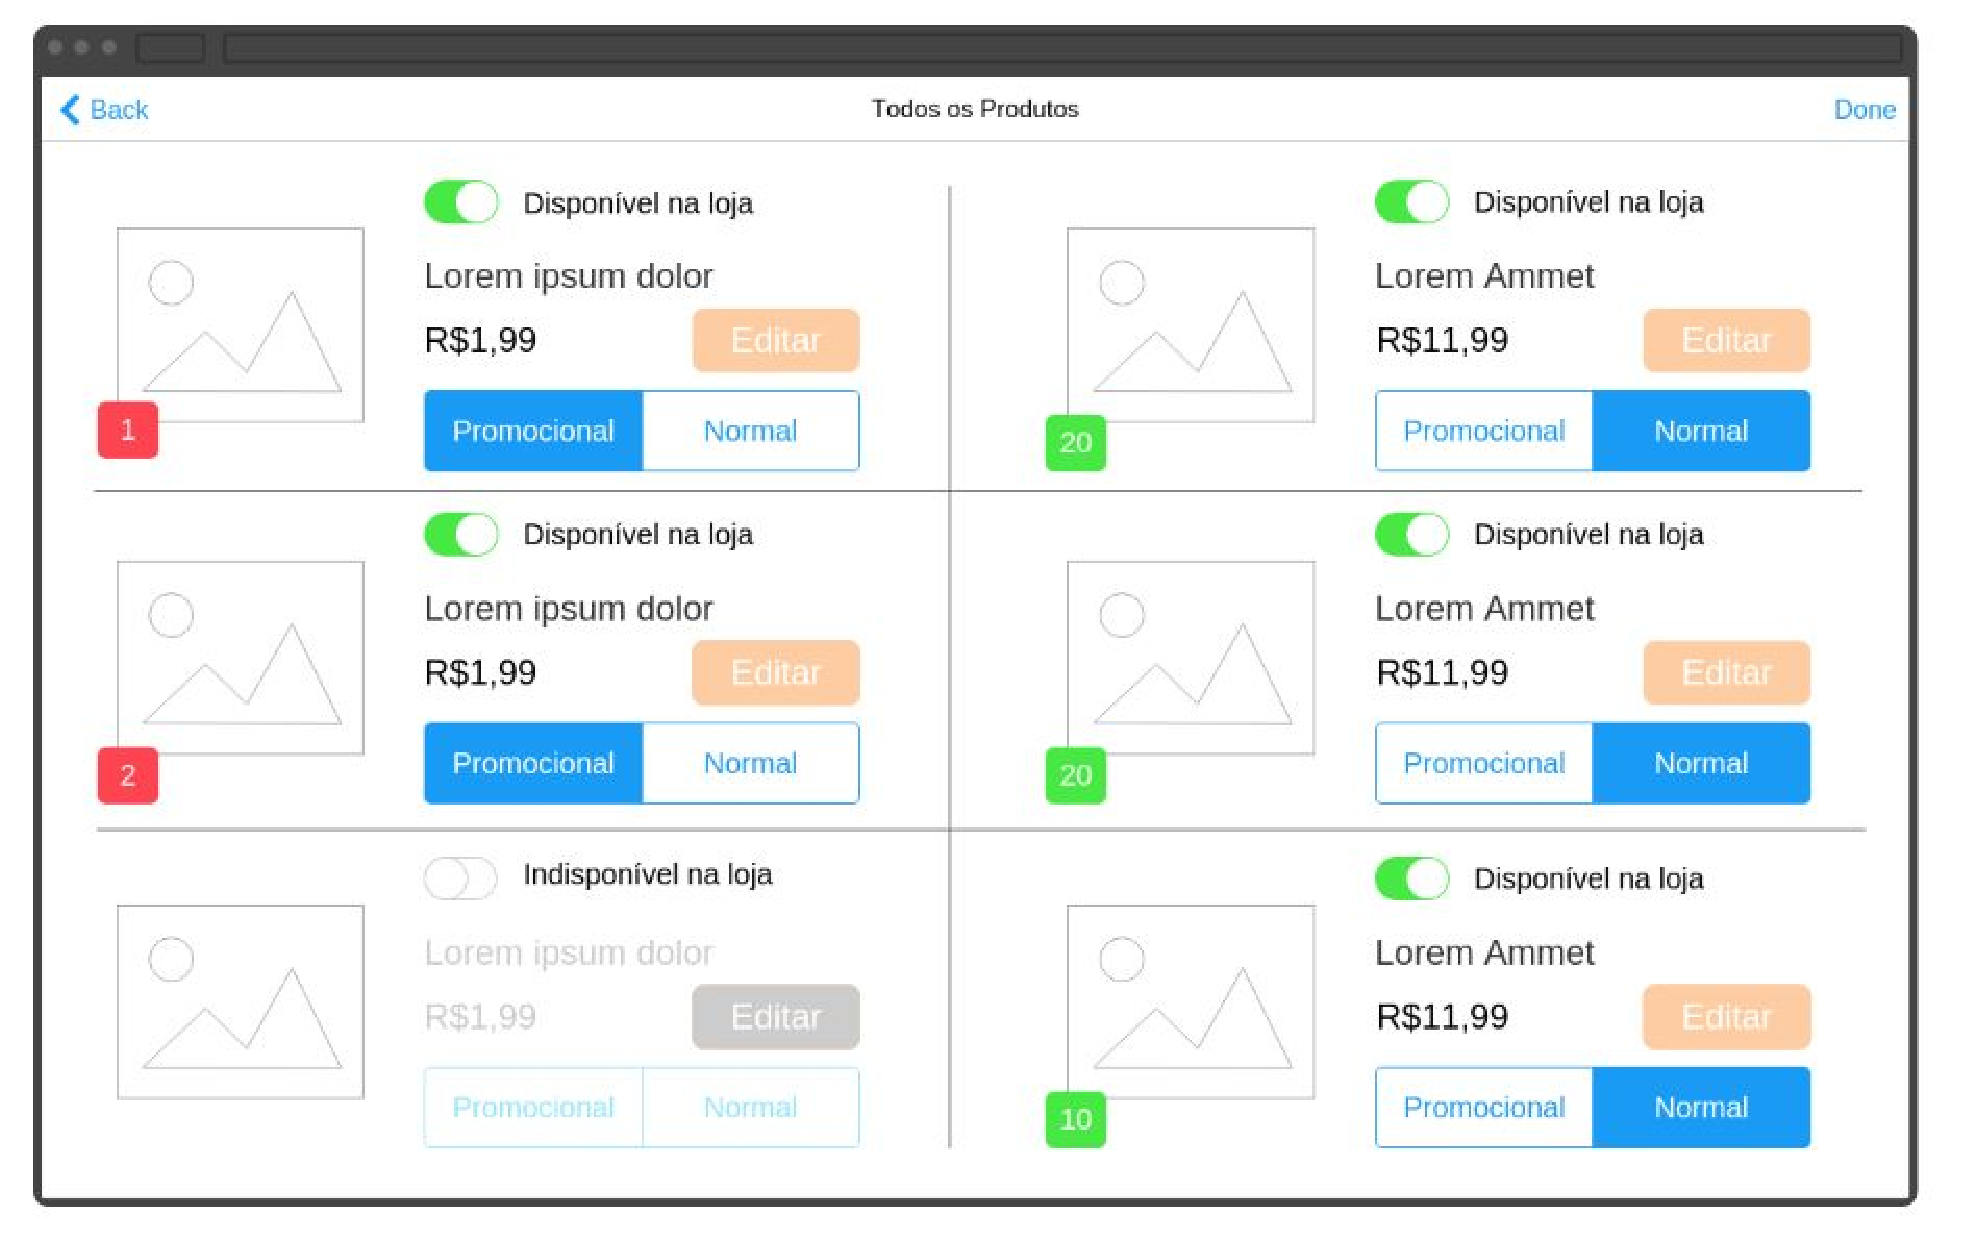
\includegraphics[width=12cm]{img/prototipos/produtos-cadastrados.eps}
\caption{Visualização de produtos cadastrados}
\label{figura:produtos_cadastrados}
\end{figure}

\begin{figure}[H]
\centering
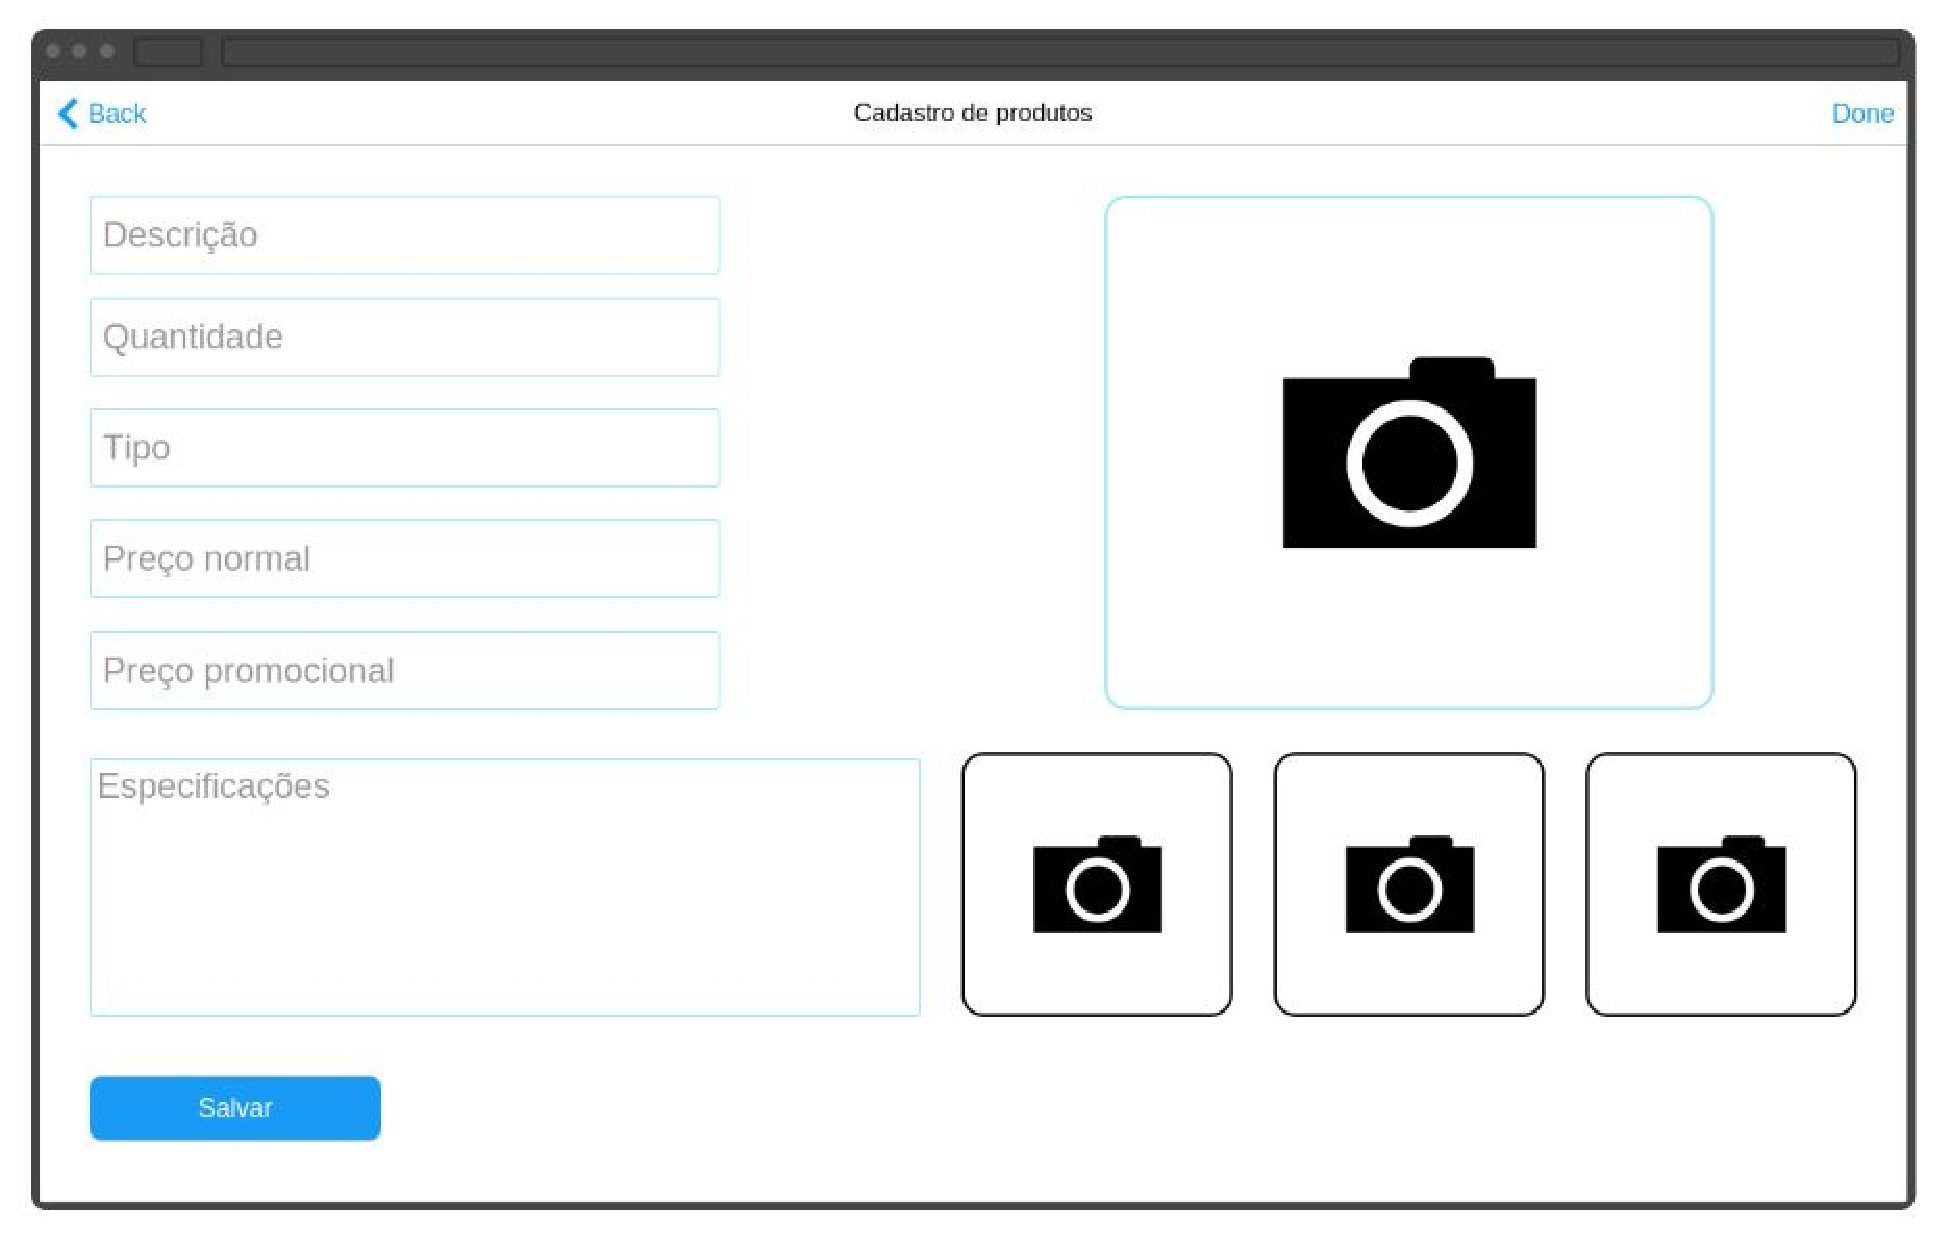
\includegraphics[width=12cm]{img/prototipos/cadastro-produto.eps}
\caption{Cadastro de produtos}
\label{figura:Cadastro_de_Produtos}
\end{figure}

\begin{figure}[H]
\centering
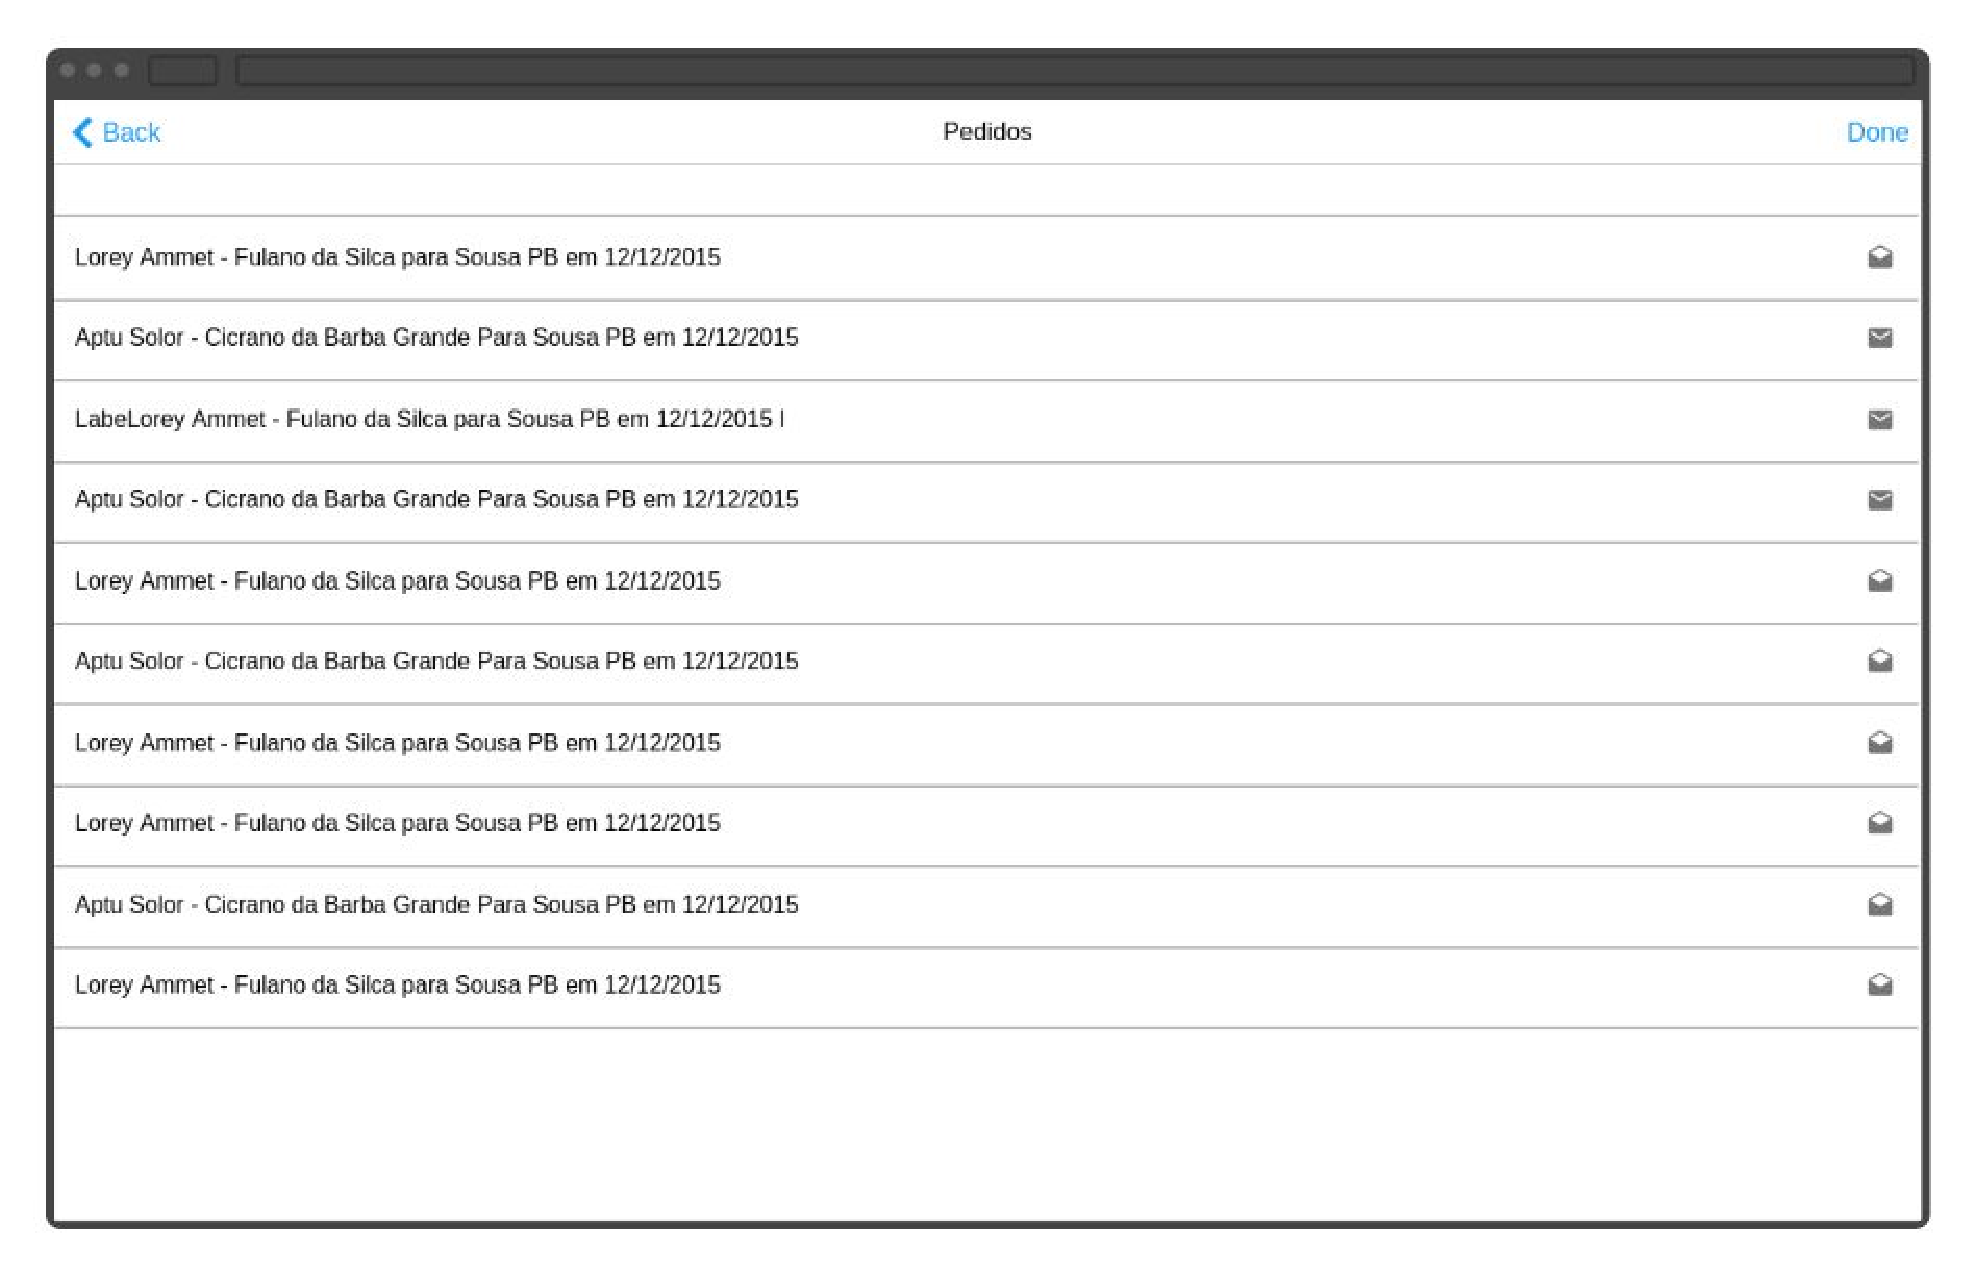
\includegraphics[width=12cm]{img/prototipos/visualizacao-pedido.eps}
\caption{Visualização de pedidos}
\label{figura:visualizacao_pedidos}
\end{figure}

\begin{figure}[H]
\centering
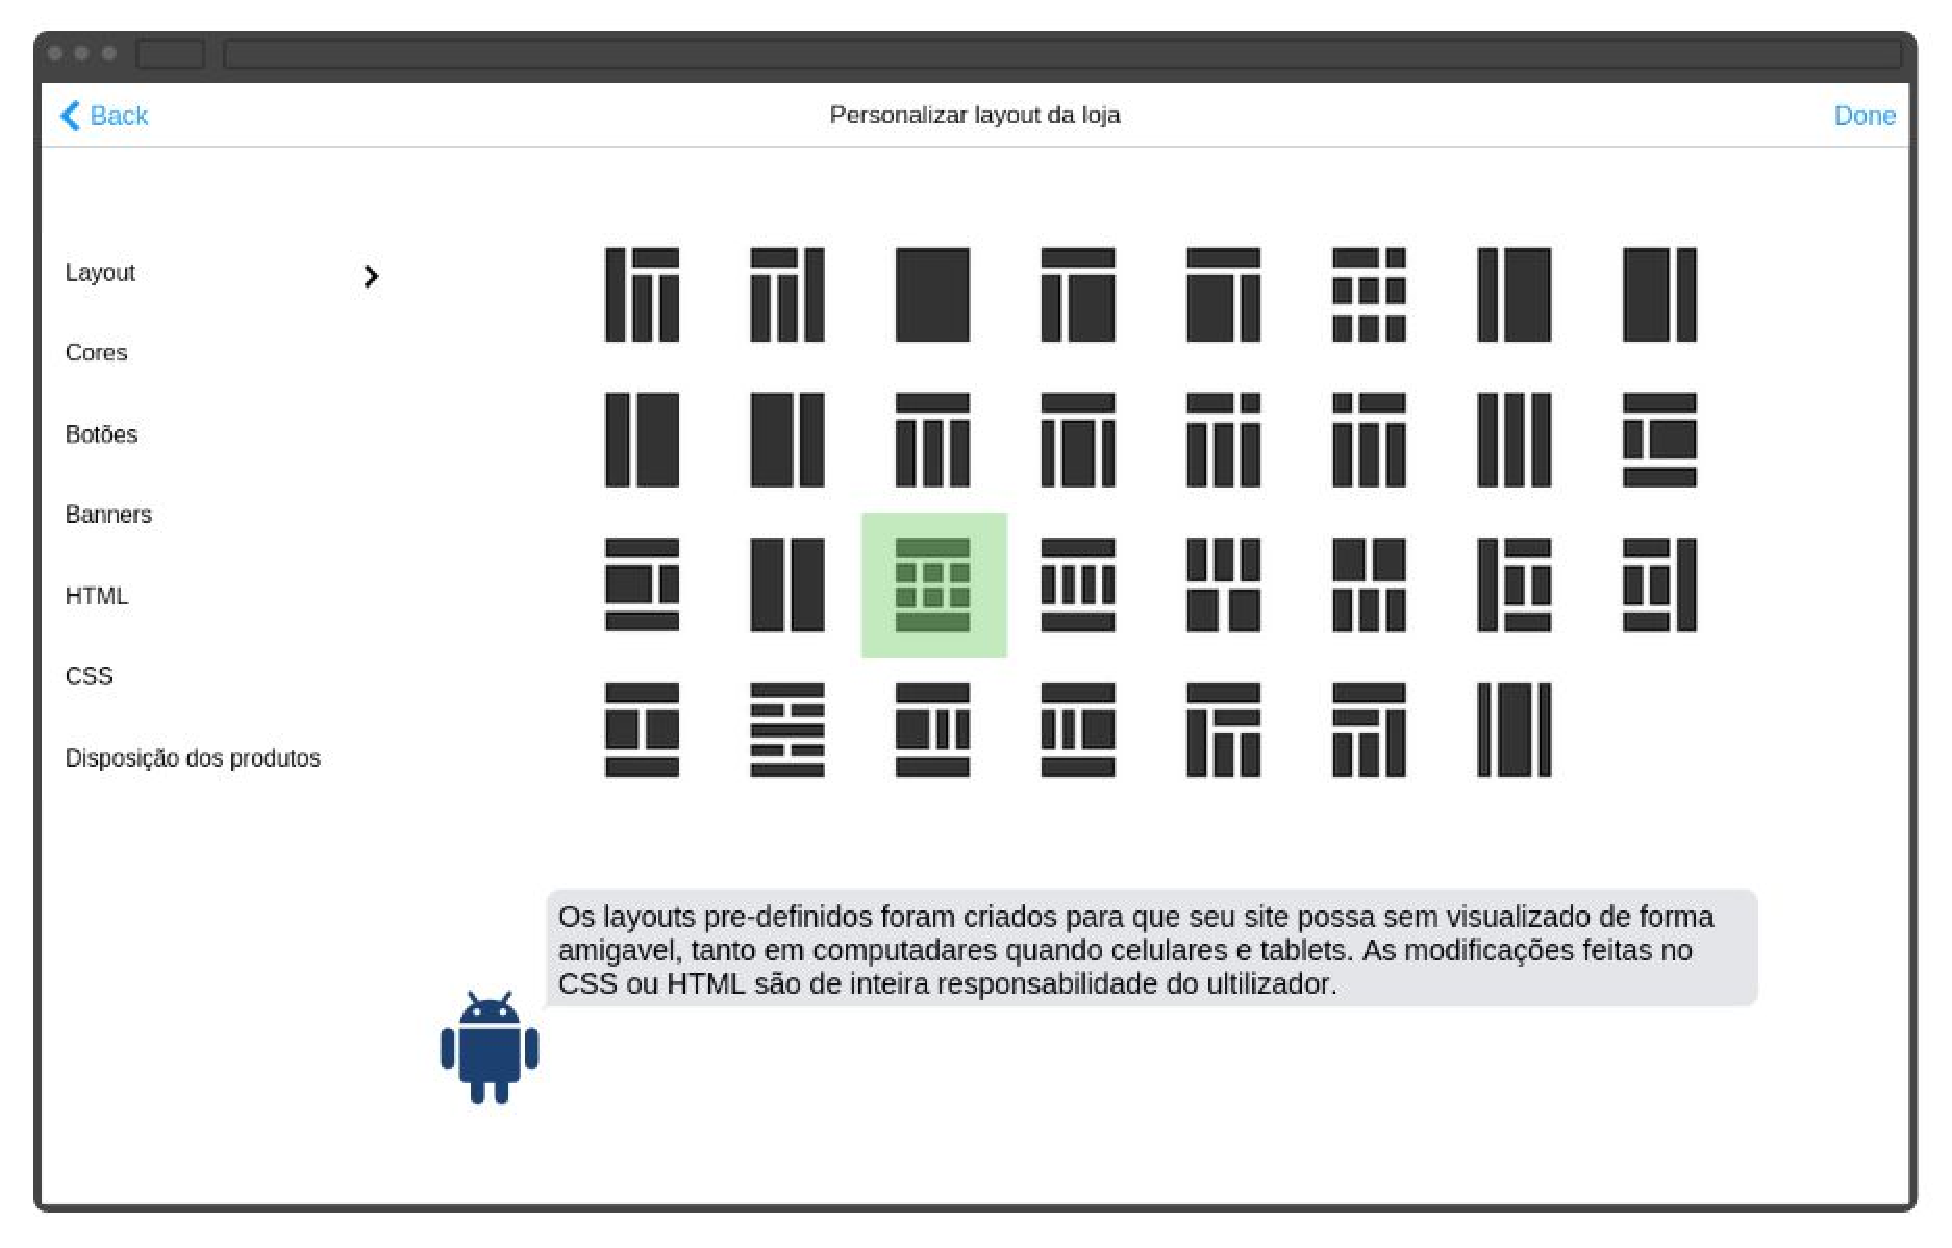
\includegraphics[width=12cm]{img/prototipos/painel-personalizacao.eps}
\caption{Painel de Personalização}
\label{figura:painel_personalizacao}
\end{figure}

\begin{figure}[H]
\centering
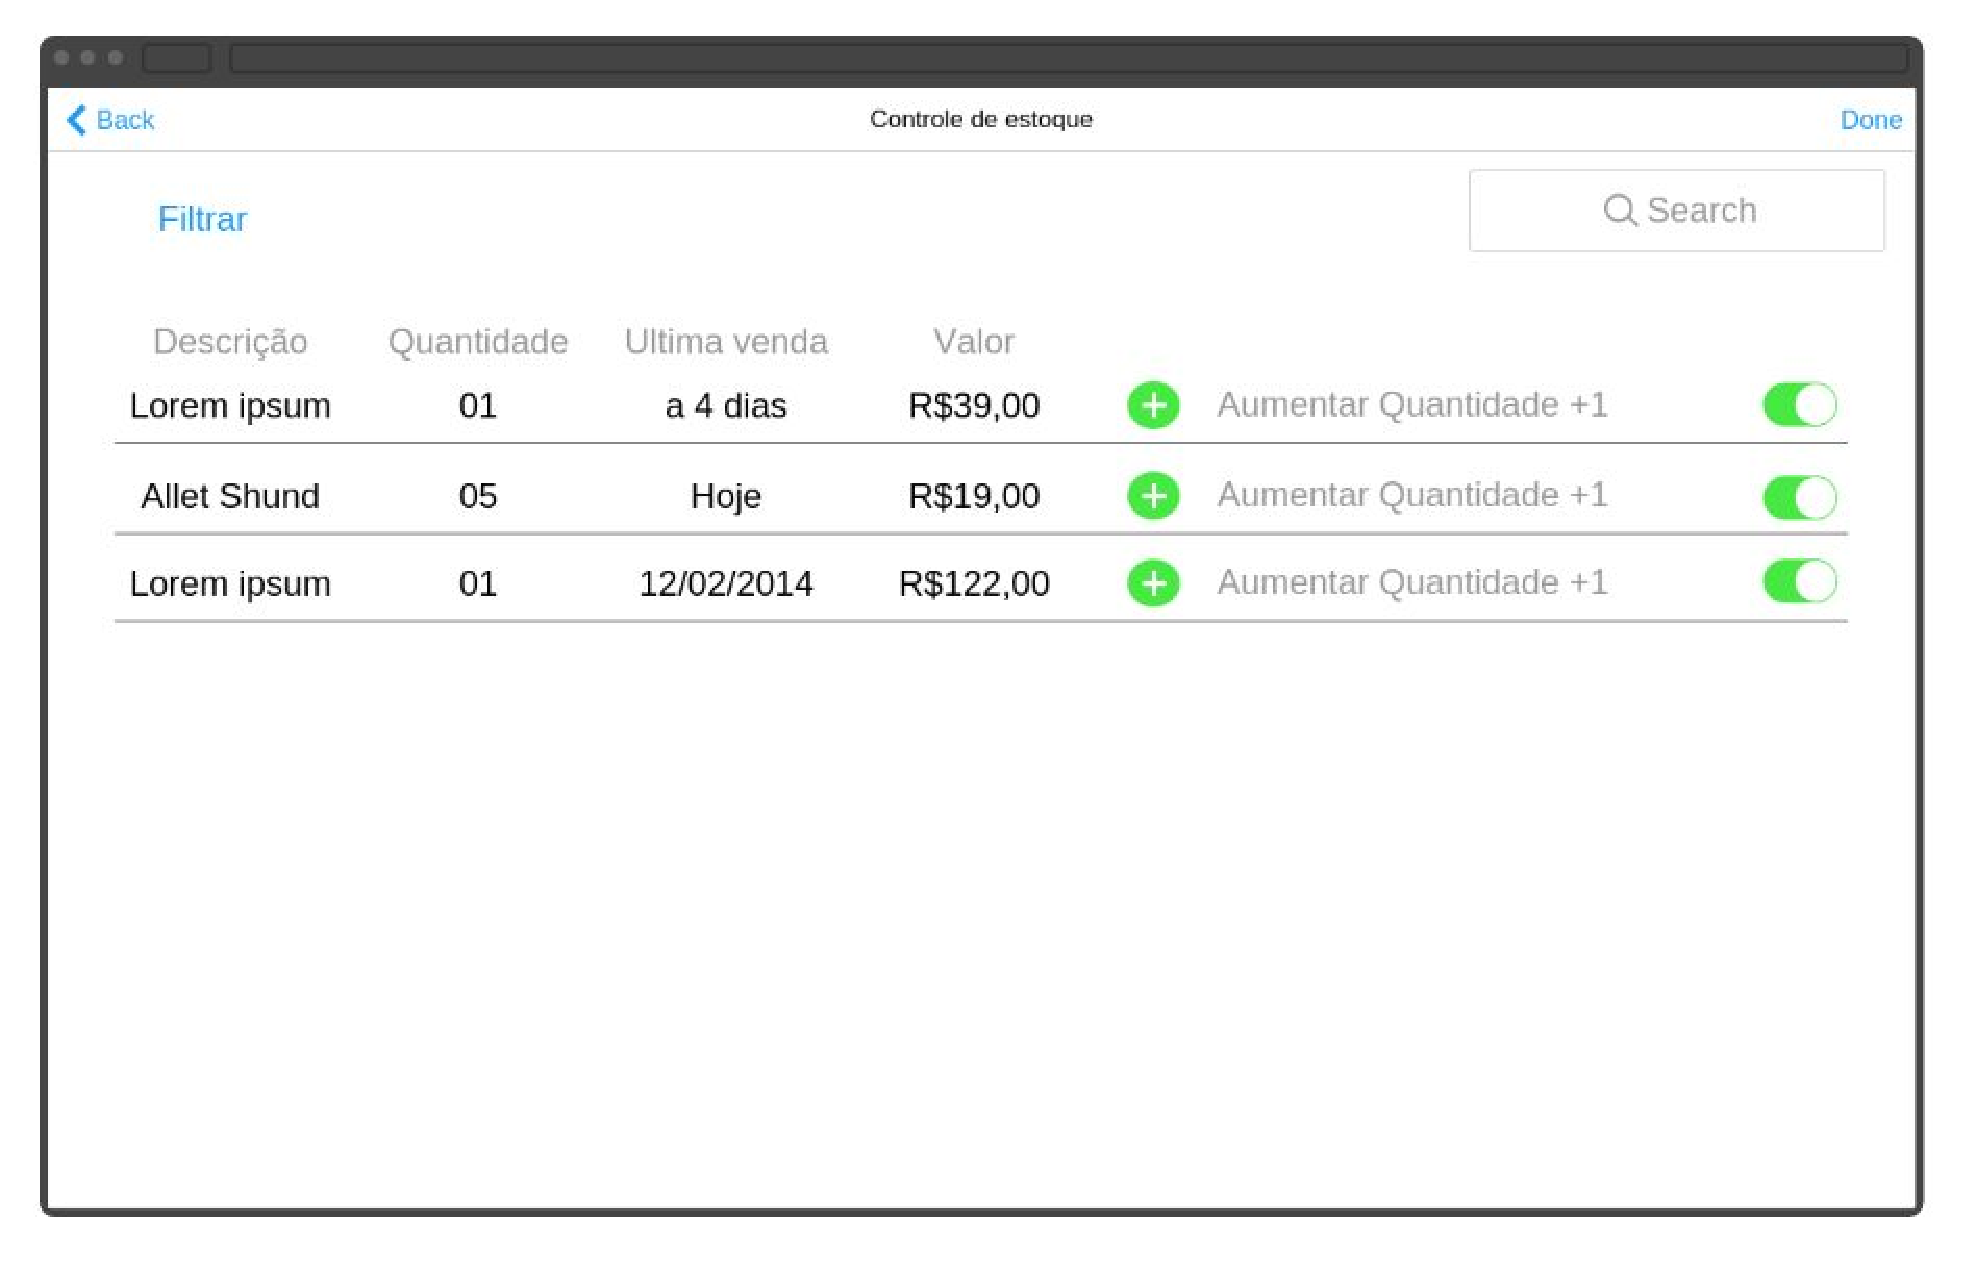
\includegraphics[width=12cm]{img/prototipos/estoque.eps}
\caption{Controle de estoque}
\label{figura:controle_estoque}
\end{figure}

% section prot_tipos (end)

\chapter{\textit{User Stories} e Testes de Aceitação} % (fold)
\label{app:user_stories_e_testes_de_aceitacao}

\begin{longtable}{|p{1.5cm}|p{3.5cm}|c|p{2cm}|p{2cm}|c|}
\caption{Alocação de Tarefas - US01}
\label{quadro:tat-us03}
\hline
\multicolumn{6}{|c|}{\textbf{\textit{User Story} 01}}\\
\hline		
\rowcolor{ballblue}
Tarefa & Descrição & Responsável & Estimativa de tempo (horas) & Tempo real (horas) & Status\\
\hline
T1 & Implementar Script para salvar um Usuário Lojista & João Marcos & 2 & 1 & Finalizado\\
\hline
T2 & Implementar Script para validar informações do usuário Lojista & João Marcos & 2 & 1 & Finalizado\\
\hline
T3 & Criar Formulário para cadastro usuários lojistas & João Marcos & 3 & 2 & Finalizado\\	
\hline
T5 & Criar página editar as informações do usuário Lojista & João Marcos & 4 & 3 & Finalizado\\	
\hline
\end{longtable}

\begin{longtable}{|l|p{11.8cm}|c|}
\caption{Teste de aceitação - US01}
\label{quadro:teste-aceitacao-us01}
\hline
\multicolumn{3}{|c|}{\textbf{\textit{User Story} 01}}\\
\hline		
\rowcolor{ballblue}
\multicolumn{2}{|c|}{Testes de aceitação} & Status\\	
\hline
TA1 & Dado que estou na página de registro de novo usuário, quando eu preencher o formulário com os dados obrigatórios de forma correta , o usuário deve ser salvo.   & Finalizado\\
\hline
TA2 & Dado que estou na página de registro de novo usuário, quando eu preencher o formulário com os dados obrigatórios de forma incorreta , o usuário não deve ser salvo e uma mensagem de erro deve ser exibida.   & Finalizado\\
\hline
TA3 & Dado que estou acessando a ficha de edição de informações sobre o Lojista, quando eu alterar alguma informação do formulário com os dados válidos, o usuário deve ser atualizado e uma mensagem de sucesso deve ser exibida.   & Finalizado\\
\hline
TA4 & Dado que estou acessando a ficha de edição de informações sobre o Lojista, quando eu alterar alguma informação do formulário com os dados inválidos, tais informações não serão salvas e uma mensagem de erro deve ser exibida.   & Finalizado\\
\hline	
\end{longtable}

\begin{longtable}{|p{1.5cm}|p{3.5cm}|c|p{2cm}|p{2cm}|c|}
\caption{Alocação de Tarefas - US01}
\label{quadro:tat-us03}
\hline
\multicolumn{6}{|c|}{\textbf{\textit{User Story} 02}}\\
\hline		
\rowcolor{ballblue}
Tarefa & Descrição & Responsável & Estimativa de tempo (horas) & Tempo real (horas) & Status\\
\hline
T1 & Implementar Script para salvar uma Loja & João Marcos & 2 & 1 & Finalizado\\
\hline
T2 & Implementar Script para validar informações do de uma Loja & João Marcos & 2 & 1 & Finalizado\\
\hline
T3 & Criar Formulário para cadastro de uma Loja & João Marcos & 3 & 2 & Finalizado\\	
\hline
T5 & Criar página editar as informações Sobre uma Loja & João Marcos & 4 & 3 & Finalizado\\
\hline
\end{longtable}

\begin{longtable}{|l|p{11.8cm}|c|}
\caption{Teste de aceitação - US02}
\label{quadro:teste-aceitacao-us02}
\hline
\multicolumn{3}{|c|}{\textbf{\textit{User Story} 02}}\\
\hline		
\rowcolor{ballblue}
\multicolumn{2}{|c|}{Testes de aceitação} & Status\\	
\hline
TA1 & Dado que estou na página de criação de uma Loja, quando eu preencher o formulário com os dados obrigatórios de forma correta , a loja ser salva.   & Finalizado\\
\hline
TA2 & Dado que estou na página criação de uma Loja, quando eu preencher o formulário com os dados obrigatórios de forma incorreta , a Loja não deve ser salva e uma mensagem de erro deve ser exibida.   & Finalizado\\
\hline
TA3 & Dado que estou acessando a página de edição de informações sobre uma Loja, quando eu alterar alguma informação do formulário com os dados válidos, a Loja deve ser atualizada e uma mensagem de sucesso deve ser exibida.   & Finalizado\\
\hline
TA4 & Dado que estou acessando a página de edição de informações sobre uma Loja, quando eu alterar alguma informação do formulário com os dados inválidos, tais informações não serão salvas e uma mensagem de erro deve ser exibida.   & Finalizado\\
\hline	
TA5 & Permitir que eu possa cadastrar mais de uma Loja no sistema.  & Finalizado\\
\hline	
\end{longtable}

\begin{longtable}{|p{1.5cm}|p{3.5cm}|c|p{2cm}|p{2cm}|c|}
\caption{Alocação de Tarefas - US03}
\label{quadro:tat-us03}
\hline
\multicolumn{6}{|c|}{\textbf{\textit{User Story} 03}}\\
\hline		
\rowcolor{ballblue}
Tarefa & Descrição & Responsável & Estimativa de tempo (horas) & Tempo real (horas) & Status\\
\hline
T1 & Implementar Script para salvar um Produto & João Marcos & 2 & 1 & Finalizado\\
\hline
T2 & Implementar Script para validar informações do produto & João Marcos & 2 & 1 & Finalizado\\
\hline
T3 & Criar Formulário para cadastro de produto & João Marcos & 3 & 2 & Finalizado\\
\hline
T4 & Criar formulário para edição de produto & João Marcos & 2 & 1 & Finalizado\\
\hline
T5 & Criar página para o estoque, exibindo as informações básicas de cada produto com sua respectiva quantidade e link para ficha do produto & João Marcos & 4 & 3 & Finalizado\\
\hline
T6 & Criar botão para exclusão de um produto na página de estoque & João Marcos & 2 & 1 & Finalizado\\
\hline
\end{longtable}

\begin{longtable}{|l|p{11.8cm}|c|}
\caption{Teste de aceitação - US03}
\label{quadro:teste-aceitacao-us03}
\hline
\multicolumn{3}{|c|}{\textbf{\textit{User Story} 03}}\\
\hline		
\rowcolor{ballblue}
\multicolumn{2}{|c|}{Testes de aceitação} & Status\\	
\hline
TA1 & Dado que estou na página de cadastro de produto, quando eu preencher o formulário com os dados obrigatórios de forma correta , o produto deve ser salvo e informado uma mensagem de sucesso.   & Finalizado\\
\hline
TA2 & Dado que estou na página de cadastro de produto, quando eu preencher o formulário com os dados obrigatórios de forma incorreta , o produto não deve ser salvo e uma mensagem de erro deve ser exibida.   & Finalizado\\
\hline
TA3 & Dado que estou acessando a ficha de edição de produto, quando eu alterar alguma informação do formulário com os dados válidos, o produto deve ser atualizado e uma mensagem de sucesso deve ser exibida.   & Finalizado\\
\hline
TA4 & Dado que estou acessando a ficha de edição de produto, quando eu alterar alguma informação do formulário com os dados inválidos, tais informações não serão salvas e uma mensagem de erro deve ser exibida.   & Finalizado\\
\hline
TA5 & Dado que estou na página de estoque, quando eu selecionar a opção excluir este produto, um diálogo de confirmação deve ser exibido. Caso confirme o produto deve ser excluído  & Finalizado\\
\hline
TA6 & Dado que estou na página de estoque, quando eu selecionar a opção excluir este produto, um diálogo de confirmação deve ser exibido. Caso não confirme o produto não deve ser excluído  & Finalizado\\
\hline
\end{longtable}

\begin{longtable}{|p{1.5cm}|p{3.5cm}|c|p{2cm}|p{2cm}|c|}
\caption{Alocação de Tarefas - US04}
\label{quadro:tat-us04}
\hline
\multicolumn{6}{|c|}{\textbf{\textit{User Story} 04}}\\
\hline		
\rowcolor{ballblue}
Tarefa & Descrição & Responsável & Estimativa de tempo (horas) & Tempo real (horas) & Status\\
\hline
T1 & Implementar Script para validar credenciais de um lojista & João Marcos & 2 & 1 & Finalizado\\
\hline
T2 & Criar página inicial contendo um menu de navegação onde o usuário poderá navegar com facilidade no sistema & João Marcos & 4 & 3 & Finalizado\\
\hline
T3 & Criar botão para sair do Sistema & João Marcos & 2 & 1 & Finalizado\\
\hline
T4 & Criar página de seleção de lojas, onde o usuário poderá escolher a loja que deseja gerenciar no momento & João Marcos & 5 & 4 & Finalizado\\
\hline
T5 & Criar página de gerenciamento específica para lojas, que será exibida ao selecionar uma Loja na T4 & João Marcos & 4 & 2 & Finalizado\\
\hline
T6 & Criar menu lateral na página de gerenciamento da loja, permitindo a navegação dentre as funcionalidades inerentes ao gerenciamento da loja & João Marcos & 2 & 1 & Finalizado\\
\hline
\end{longtable}

\begin{longtable}{|l|p{11.8cm}|c|}
\caption{Teste de aceitação - US04}
\label{quadro:teste-aceitacao-us04}
\hline
\multicolumn{3}{|c|}{\textbf{\textit{User Story} 04}}\\
\hline		
\rowcolor{ballblue}
\multicolumn{2}{|c|}{Testes de aceitação} & Status\\	
\hline
TA1 & Dado que estou na página de login, quando eu preencher o formulário com os dados obrigatórios de forma correta , ser redirecionado para a página inicial do sistema.   & Finalizado\\
\hline
TA2 & Dado que estou na página de login, quando eu preencher o formulário com os dados obrigatórios de forma incorreta , não posso ser redirecionado para o sistema e uma mensagem de erro deve ser exibida.   & Finalizado\\
\hline
TA3 & Dado que estou logado, quando clicar no botão sair, devo ser desconectado do sistema, onde terei que fazer login novamente caso queira entrar no sistema novamente.   & Finalizado\\
\hline
TA4 & Dado que estou na página de seleção de lojas, quando selecionar uma loja, devo ser redirecionado  para página inicial de gerenciamento da Loja selecionada.  & Finalizado\\
\hline
TA5 & Dado que estou logado, quando eu selecionar uma opção do menu lateral, devo ser redirecionado para página especificada  & Finalizado\\
\hline	
\end{longtable}

% chapter user_stories_e_testes_de_aceita_o (end)

\chapter{Plano de Iteração} % (fold)
\label{apdc:plano_de_itercao}

\begin{table}[H]
\centering
\caption{\textit{Release} 01}
\label{qua:release01}
\begin{tabular}{|lc|c|}
\rowcolor{ballblue}
\hline
\textbf{Release 01} & & Gerente - João Marcos \\
\hline
Iteração & \textit{\textit{User Stories}} & Período\\
\hline
Iteração 1    & US01           & 04/06/2015 - 11/06/2015\\
Iteração 2    & US02           & 12/06/2015 - 18/06/2015\\
\hline
\rowcolor{ballblue}
\hline				
\end{tabular}
\end{table}

\begin{table}[H]
\centering
\caption{\textit{Release} 02}
\label{qua:release02}
\begin{tabular}{|lc|c|}
\rowcolor{ballblue}
\hline
\textbf{Release 02} & & Gerente - João Marcos \\
\hline
Iteração & \textit{\textit{User Stories}} & Período\\
\hline
Iteração 3    & US03 		   & 19/06/2015 - 02/07/2015\\
Iteração 4    & US04 		   & 03/07/2015 - 16/07/2015\\
\hline
\end{tabular}
\end{table}

\begin{table}[H]
\centering
\caption{\textit{Release} 03}
\label{qua:release03}
\begin{tabular}{|lc|c|}
\rowcolor{ballblue}
\hline
\textbf{Release 02} & & Gerente - João Marcos \\
\hline
Iteração & \textit{\textit{User Stories}} & Período\\
\hline
Iteração 5    & US06, US08    & 02/12/2015 - 14/12/2015\\
Iteração 6    & US09, US10	  & 15/12/2015 - 21/12/2015\\
\hline
\end{tabular}
\end{table}

\begin{table}[H]
\centering
\caption{\textit{Release} 04}
\label{qua:release04}
\begin{tabular}{|lc|c|}
\rowcolor{ballblue}
\hline
\textbf{Release 04} & & Gerente - João Marcos \\
\hline
Iteração & \textit{\textit{User Stories}} & Período\\
\hline
Iteração 7    & US07  & 10/02/2016 - 15/02/2016\\
Iteração 8    & US11  & 16/02/2016 - 28/02/2016\\
\hline
\end{tabular}
\end{table}

\begin{table}[H]
\centering
\caption{\textit{Release} 05}
\label{qua:release05}
\begin{tabular}{|lc|c|}
\rowcolor{ballblue}
\hline
\textbf{Release 04} & & Gerente - João Marcos \\
\hline
Iteração & \textit{\textit{User Stories}} & Período\\
\hline
Iteração 9    & US05  & 12/03/2016 - 02/04/2016\\
\hline
\end{tabular}
\end{table}

% chapter plano_de_itera_o (end)

\chapter{Telas do Sistema} % (fold)
\label{cha:telas_do_sistema}

% chapter telas_do_sistema (end)

\end{document}
